\chapter{等価原理からテンソルへ}

一般相対性理論は通常GRと略されるが、特殊相対性理論がSRと呼ばれることはほとんどない。略称そのものよりも、最初から始めるという決断のほうが重要である。最も直接的な道筋はアインシュタインがたどった道である。すなわち、エレベーターの中で感じ取れるほど単純な物理的観察から出発し、その帰結が避けられなくなるまで押し進め、その後に初めて幾何学を導入するのである。

最初の観察は等価原理である。重力と加速度は局所的に区別できない。局所的にという言葉は、やがてこの主張のほぼ全重量を担うことになる。しかしそれを限定する前に、限定されていない主張がすでに何をなしうるかを見ておくべきである。

\section{座標変換としてのエレベーター}

教科書ではアインシュタインのエレベーターをロケット船に置き換えることが多い。ここではエレベーターのほうが好ましい。その加速度が身近だからである。地面に固定された系で高さを\(z\)で測り、エレベーターの床からの高さを\(z'\)で測ることにする。床の高さが\(L(t)\)であるとき、同じ事象の座標は
\begin{equation}
 z'=z-L(t),\qquad t'=t,\qquad x'=x.
\label{eq:elevator-map}
\end{equation}
となる。エレベーターは横に滑らないので、水平座標は変わらない。\(t'=t\)と置くことは、当面、特殊相対性理論を意図的に抑えているのである。

\begin{classroomqa}
\audiencequestion{一般相対性理論の講義が、特殊相対性理論を無視することから始まるとはどういうことか。}
\lecturerresponse{重力が重要でありながら、すべての速度が\(c\)に比べて小さいままである領域が存在する。したがって、重力と--加速度の関係はニュートン力学において切り離して扱い、その後でミンコフスキー幾何学と組み合わせることができる。これは段階的な選択であり、最終的な理論が非相対論的であるという主張ではない。\lecturetimestamp{00:05:33}}
\end{classroomqa}

二つの慣性系に対して、エレベーターは一様に運動し、
\begin{equation}
 L(t)=vt,\qquad z'=z-vt.
\label{eq:galilean-elevator}
\end{equation}
となる。原点は\(t=0\)で一致するように選んである。黒板にはエレベーターのスケッチを三つの座標関係のそばに置き、記号がその物理的意味を失わないようにしてある。

\begin{figure}[H]
\centering
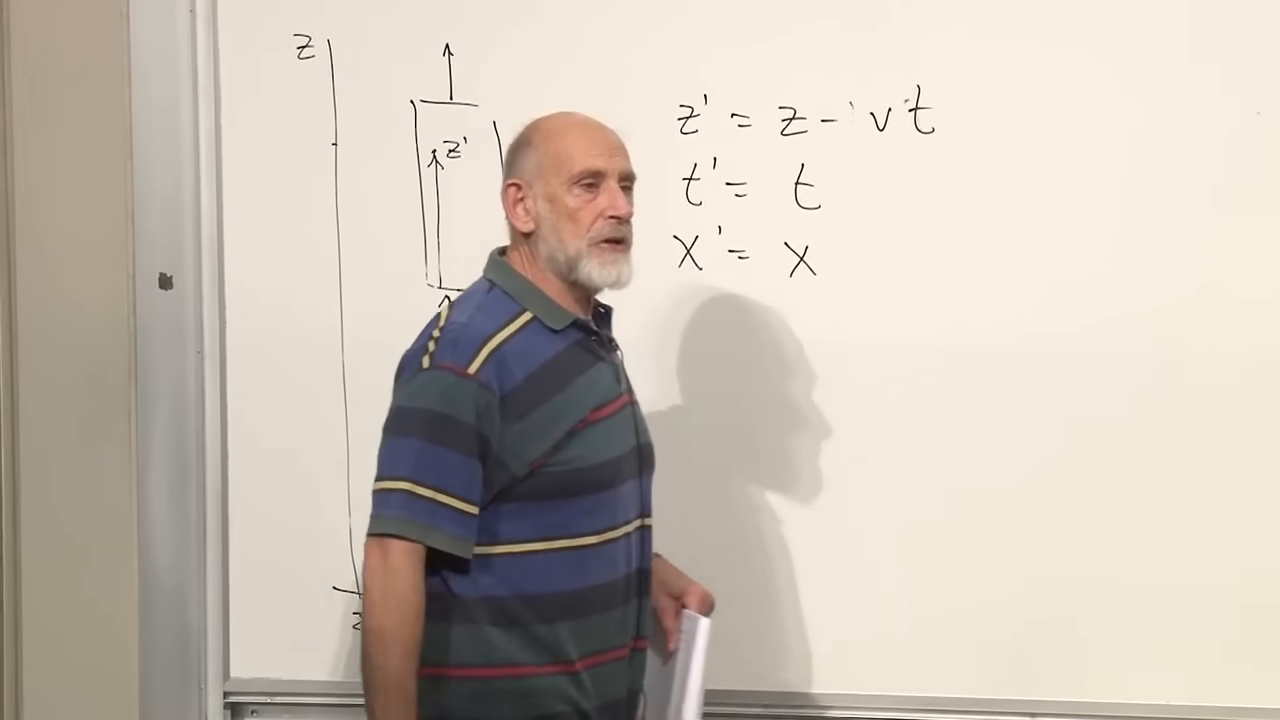
\includegraphics[width=\linewidth]{lecture_01_figure_01.png}
\caption{一様速度への特殊化\(L(t)=vt\)の後のエレベーター座標。}
\par\smallskip
\textit{講義の系: 00:09:10。}
\end{figure}

ニュートンの法則の鉛直成分だけを考えると、
\begin{equation}
 F=m\ddot z.
\label{eq:newton-unprimed}
\end{equation}
となる。力はロープから来ても、電場から来ても、その他の通常の相互作用から来てもよい。\eqref{eq:galilean-elevator}を二度微分すると
\(\ddot z'=\ddot z\)となり、したがって
\begin{equation}
 F=m\ddot z'.
\label{eq:newton-primed-inertial}
\end{equation}
となる。法則の形は変わらない。この初等的な計算は、慣性系の等価性の実際の内容を明らかにする。すなわち、線形な座標変換は一様運動を一様運動へ写すのである。

\begin{figure}[H]
\centering
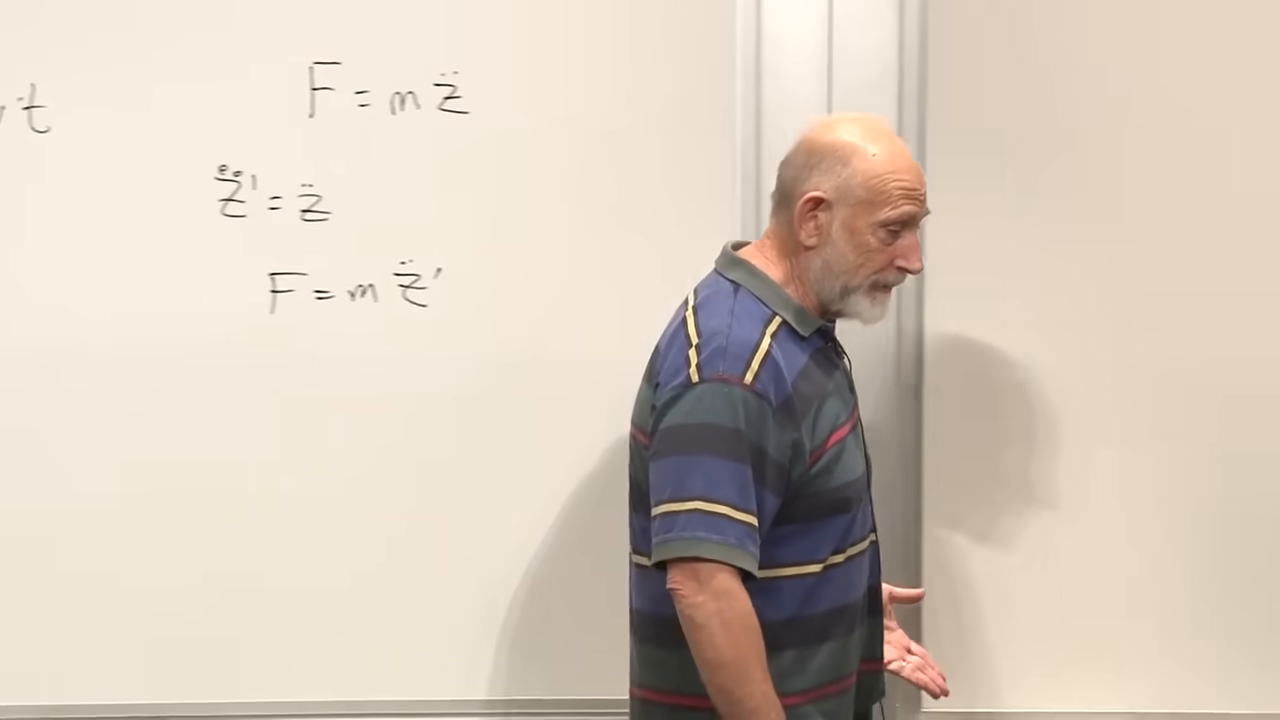
\includegraphics[width=\linewidth]{lecture_01_figure_02.png}
\caption{一様に運動する二つの座標系におけるニュートンの方程式。}
\par\smallskip
\textit{講義の系: 00:11:50。}
\end{figure}

次にエレベーターを一定の\(g\)で上向きに加速する:
\begin{equation}
 L(t)=\frac12gt^2,\qquad
 \dot L=gt,\qquad
 \ddot L=g.
\end{equation}
座標変換は
\begin{equation}
 z'=z-\frac12gt^2,
\qquad
 \ddot z'=\ddot z-g.
\label{eq:accelerated-map}
\end{equation}
となる。ニュートンの法則に代入すると
\begin{equation}
 F=m(\ddot z'+g),
\qquad
 m\ddot z'=F-mg.
\label{eq:fictitious-gravity}
\end{equation}
が得られる。この導出には有用な符号の実地確認が含まれている。\(+mg\)はまず加速度の側に現れ、力の側に移したときに初めて\(-mg\)となる。最終的な向きは、床が上向きに加速している系において下向きである。

\begin{figure}[H]
\centering
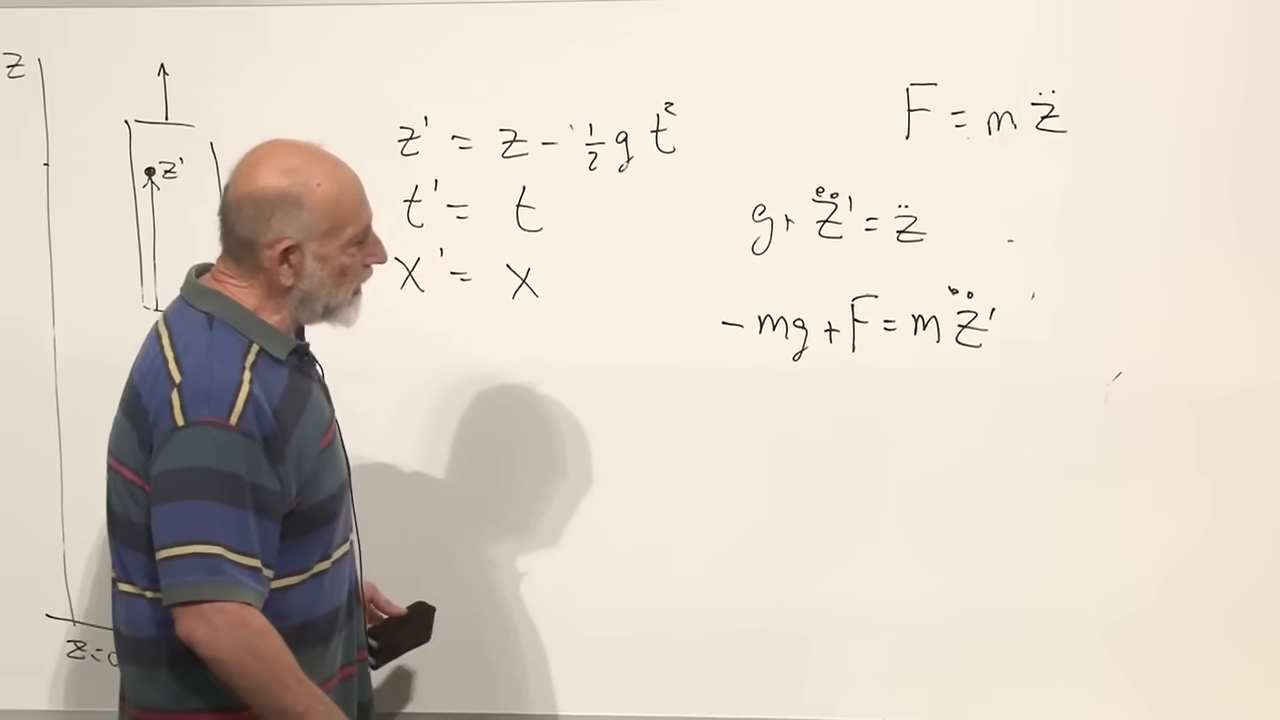
\includegraphics[width=\linewidth]{lecture_01_figure_03.png}
\caption{加速された変換と、その結果生じる見かけの力\(-mg\)。}
\par\smallskip
\textit{講義の系: 00:15:35。}
\end{figure}

新しい項が重力的に見えるのには正確な理由がある。それは質量に比例する。慣性応答もまた質量に比例するので、運動方程式から質量が消える。自由落下する物体は、その質量によらず同じ軌道をたどる。たとえば地球の軌道は、試験体近似において、地球自身の質量ではなく、太陽の場におけるその位置と速度によって決まる。

アインシュタイン以前には、この類似は単なる珍奇な事実として片付けられていた。アインシュタインはむしろそれを原理へと昇格させた。すなわち、いかなる局所的な力学実験も、一様な重力場と適切に加速された系とを区別できない、というのである。

\section{直線、曲線座標、そして光}

\(t\)を縦軸に、\(z\)を横軸にプロットする。\(z'=z-vt\)に対して、\(z'\)が一定の線は平行な直線である。座標変換が線形であるため、直線的な世界線は直線のままである。

\begin{figure}[H]
\centering
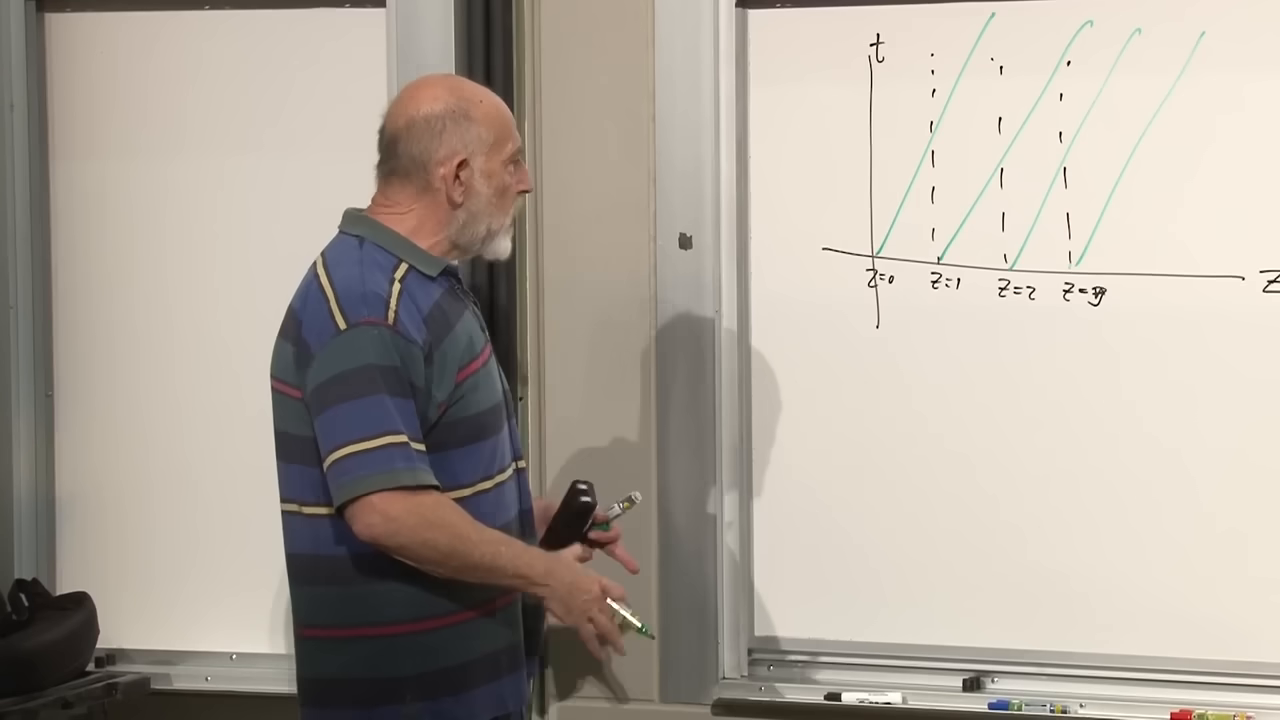
\includegraphics[width=\linewidth]{lecture_01_figure_04.png}
\caption{一様に運動する座標に対する線形な時空格子。}
\par\smallskip
\textit{講義の系: 00:19:45。}
\end{figure}

加速された写像では、一定の\(z'\)の線は次を満たす。
\begin{equation}
 z=z'+\frac12gt^2.
\end{equation}
それは横倒しになった放物線である。運動を時間的に過去へ延長すると、上昇しながら減速し、向きを変え、その後上向きに加速するエレベーターが得られる。隣接する各々の一定の\(z'\)の線は、水平方向にずれた同じ放物線である。

\begin{figure}[H]
\centering
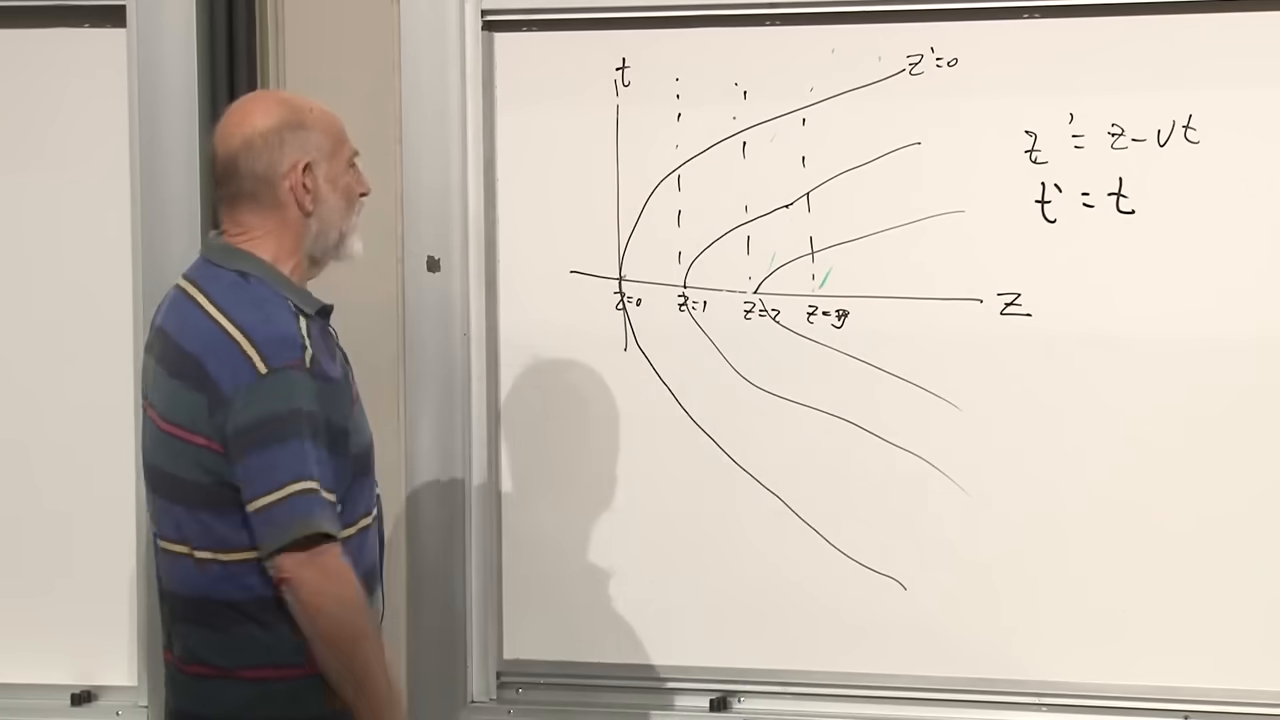
\includegraphics[width=\linewidth]{lecture_01_figure_05.png}
\caption{一様に加速された座標系に対する一定の\(z'\)曲線。}
\par\smallskip
\textit{講義フレーム：00:22:25。}
\end{figure}

これが最初の幾何学的な手がかりである。特殊相対性理論は線形なローレンツ変換を用い、それは直線的な時空の線を直線的な時空の線へと移す。加速度を表すには、したがって重力を模倣するには、時空座標の曲線的な変換が必要である。

アインシュタインはこの一見ささやかな点を用いて、まったくささやかではない問いに答えた。すなわち、重力は光に影響を与えるか、という問いである。\(t=0\)において、エレベーター系と地面系を互いに瞬間的に静止させ、水平な光線をエレベーターを横切って送る。加速されていない系では、
\begin{equation}
 x=ct,\qquad z=0.
\end{equation}
\(z=z'+\tfrac12gt^2\)を用いると、同じ光線はエレベーター座標において次に従う。
\begin{equation}
 z'=-\frac12gt^2
    =-\frac{g}{2c^2}x^2.
\label{eq:accelerated-light}
\end{equation}
光線は慣性系では直線であり、加速系では曲がっている。加速度と重力が局所的に等価であるならば、重力場は光を曲げなければならない。この議論は、重力の場の方程式が書かれる前に、その効果を確立する。

\begin{figure}[H]
\centering
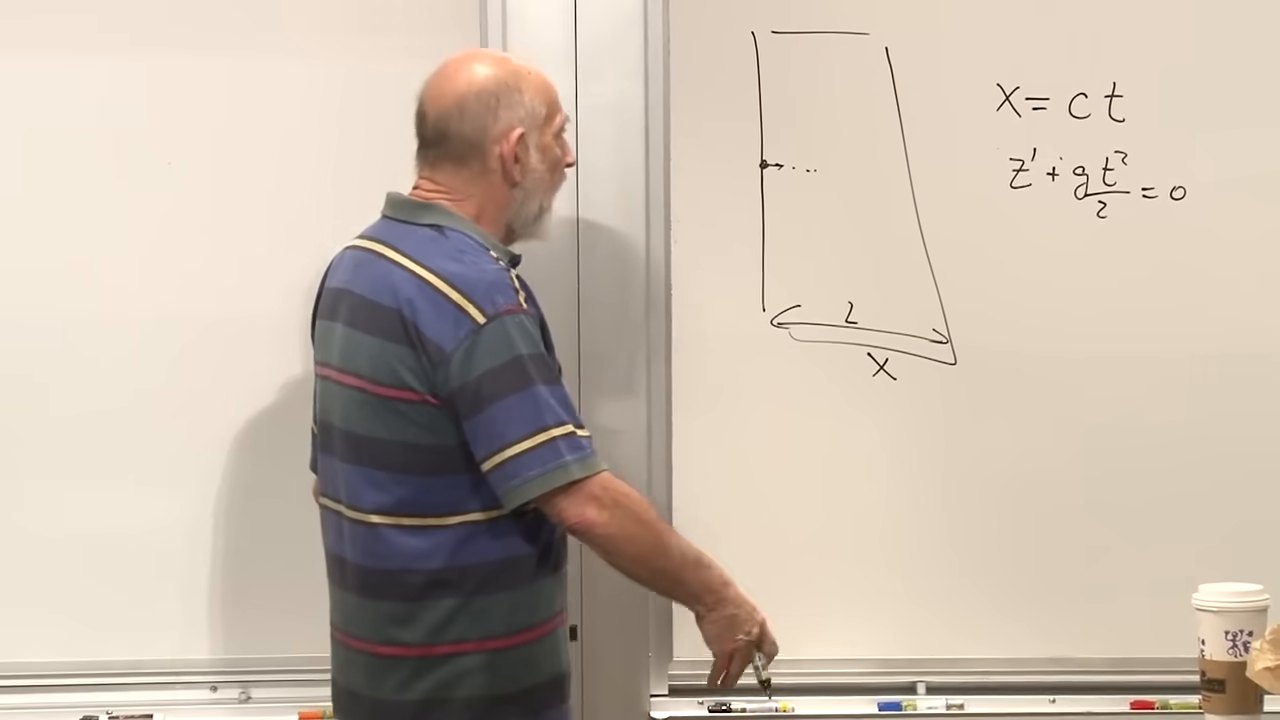
\includegraphics[width=\linewidth]{lecture_01_figure_06.png}
\caption{加速系における水平な光線とその曲がった軌道。}
\par\smallskip
\textit{講義フレーム：00:28:10。}
\end{figure}

\section{変換によって消し去ることのできないもの}

加速系は見かけ上の一様な重力場を作り出すことができる。だからといって、すべての重力場が座標の産物であるということにはならない。恒星の場は半径方向内側を向いている。ある一点の近くにある小さな自由落下する実験室は局所的な加速度を消すことができるが、同じ変換は恒星のすべての側でその場を消すことはできない。

\begin{figure}[H]
\centering
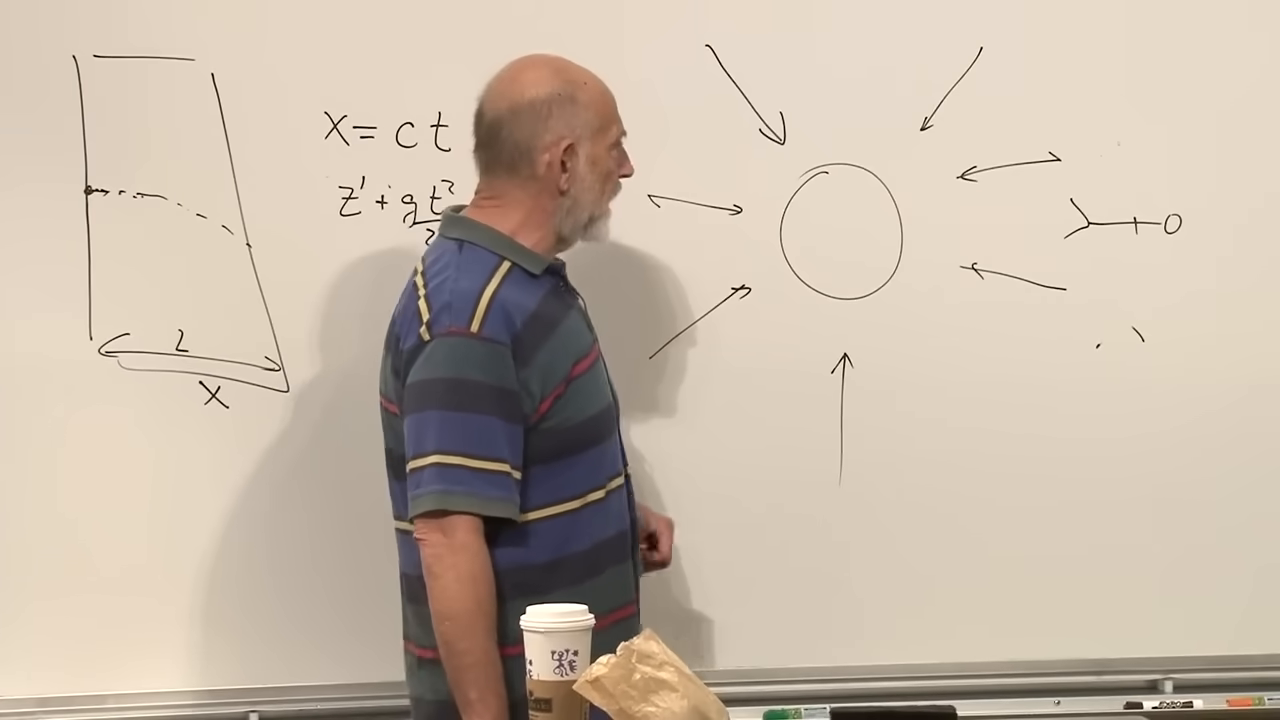
\includegraphics[width=\linewidth]{lecture_01_figure_07.png}
\caption{潮汐加速度を露わにするために用いられる動径方向の場と拡がった落下物体。}
\par\smallskip
\textit{講義フレーム：00:32:50。}
\end{figure}

障害となるのは潮汐力である。二千マイルの人間が足から先に落下すると想像せよ。彼の足は源に近く、頭よりも強く加速されるので、彼は引き伸ばされる。彼を横向きにすると、反対側の内側方向は互いに向かう成分をもつので、彼は押しつぶされる。ニュートン的な言葉では、\(\xi^j\)だけ離れた隣接する点は相対加速度
\begin{equation}
 \delta a^i \simeq \partial_j g^i\,\xi^j.
\label{eq:newtonian-tide}
\end{equation}
を得る。座標加速度は取り除くことができる。拡がった自由落下物体にわたる相対加速度は取り除くことができない。

\begin{classroomqa}
\audiencequestion{頭と足で異なるロケットエンジンが引き伸ばしを模擬し、したがって潮汐場を模擬することができるだろうか。}
\lecturerresponse{加えられたエンジンは確かに物体に応力を及ぼすことができるが、それはその部分に異なるように作用する実在の非重力力である。座標の変更だけでは、隣接する自由落下粒子の間に不変な相対加速度を生み出すことはできない。この診断は、強制されていない自由落下に関するものであり、別々のロケットによって駆動される物体に関するものではない。
\lecturetimestamp{00:36:51}}
\end{classroomqa}

それにもかかわらず、曲がった座標は見かけの場をかなり複雑に見せることができる。系は鉛直方向に加速しながら水平方向に振動し、両方の成分をもつ時間依存の見かけの場を生み出すかもしれない。普通の極座標でさえ示唆に富む例を与える。直線的なデカルト座標の線上を運動する自由粒子は、まず減少する\(r(t)\)をもち、最小半径に達し、その後増加する\(r(t)\)をもつ。\(r(t)\)と\(\theta(t)\)だけを与えられた者は、外向きの斥力を推論するかもしれない。これらの座標の回転する変種では、遠心力とコリオリの項が現れる。それらは質量に比例するので重力的に見えるが、自由落下物体に不変な潮汐歪みを残さない。

\begin{classroomqa}
\audiencequestion{運動が角度座標や極座標で記述されるとどうなるか。}
\lecturerresponse{非線形な座標記述は、直線的な自由軌道を\(r=0\)から斥けられているかのように見せる。その実効的な遠心力は座標力である。慣性デカルト系に戻るとそれは消え、潮汐的な歪みは現れない。
\lecturetimestamp{00:37:56}}
\end{classroomqa}

\begin{figure}[H]
\centering
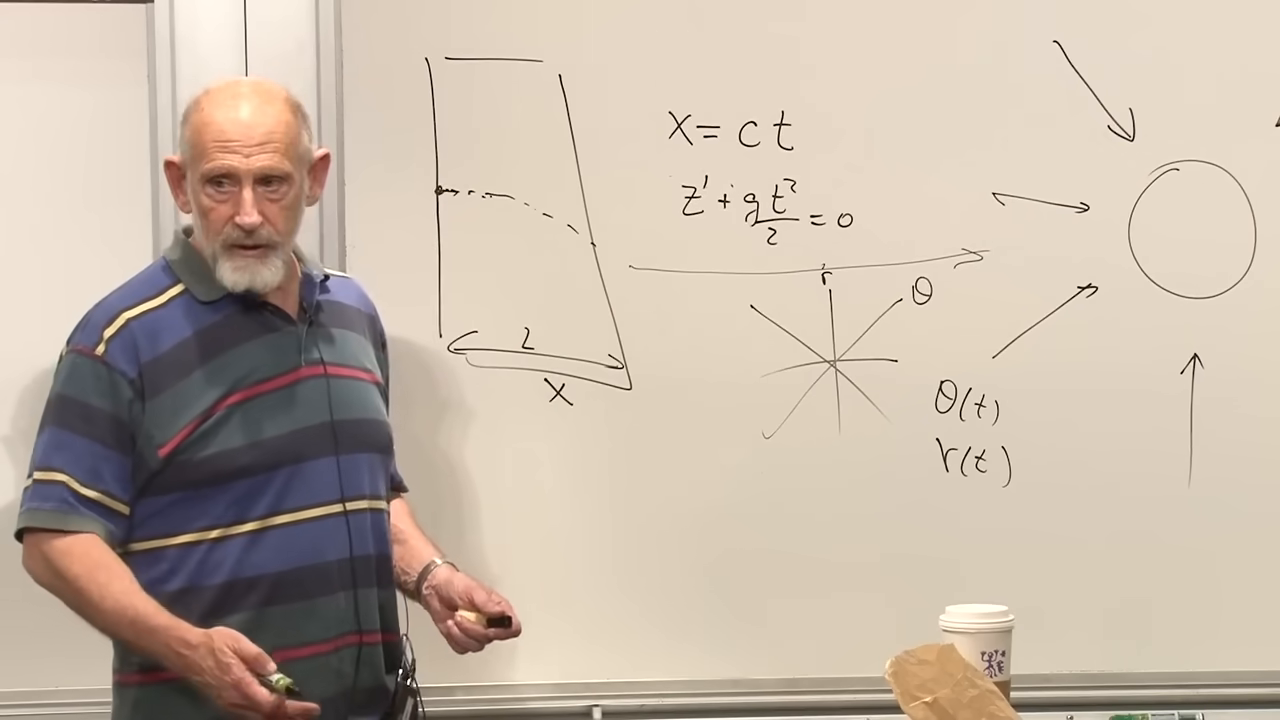
\includegraphics[width=\linewidth]{lecture_01_figure_08.png}
\caption{黒板に\(r(t)\)と\(\theta(t)\)が記された、直線軌道の極座標による記述。}
\par\smallskip
\textit{講義フレーム：00:40:20。}
\end{figure}

\begin{classroomqa}
\audiencequestion{複数の重力源が互いに打ち消し合い、潮汐力がまったく残らないということはあり得るか。}
\lecturerresponse{力は選んだ一点で打ち消し合うことはできるが、場の値の打ち消しは、一般にはその空間微分を打ち消さない。どの一つの源の近くでも、隣接する軌道は依然として異なる加速度を得る。曲率が真に存在しないためには、潮汐的な診断量がその領域全体で消えなければならず、単に一点での正味の力が消えるだけでは足りない。\lecturetimestamp{00:42:16}}
\end{classroomqa}

\begin{classroomqa}
\audiencequestion{潮汐力は操作的にどのように測定されるのか。}
\lecturerresponse{結晶のような広がりをもつ物体を自由落下させ、一方向に引き伸ばし、別の方向に圧縮する応力とひずみを探す。それらの変形は測定可能であり、座標の名前を変えても消えない。\lecturetimestamp{00:44:38}}
\end{classroomqa}

\begin{classroomqa}
\audiencequestion{メリーゴーラウンドに乗った二千マイルの人は、動径方向の潮汐効果を感じるだろうか。}
\lecturerresponse{カルーセルに固定された人は支持力を受け、実際に頭痛を起こすかもしれない。しかし試験物体は自由落下していなければならない。その軌道は回転座標では複雑に見えるが、慣性系では応力のない直線軌道のままであり、したがって不変な潮汐力はゼロである。
\lecturetimestamp{00:45:07}}
\end{classroomqa}

\begin{classroomqa}
\audiencequestion{落下する物体を傾けて、引き伸ばしと圧縮が打ち消し合うようにできるか。}
\lecturerresponse{いかなる単一の向きも、変形の全体を取り除くことはない。動径方向の場は一つの主方向に沿って引き伸ばし、横方向に沿って圧縮する。すべての方向に有限の広がりをもつ物体は、その完全なパターンを経験する。\lecturetimestamp{00:47:10}}
\end{classroomqa}

\begin{figure}[H]
\centering
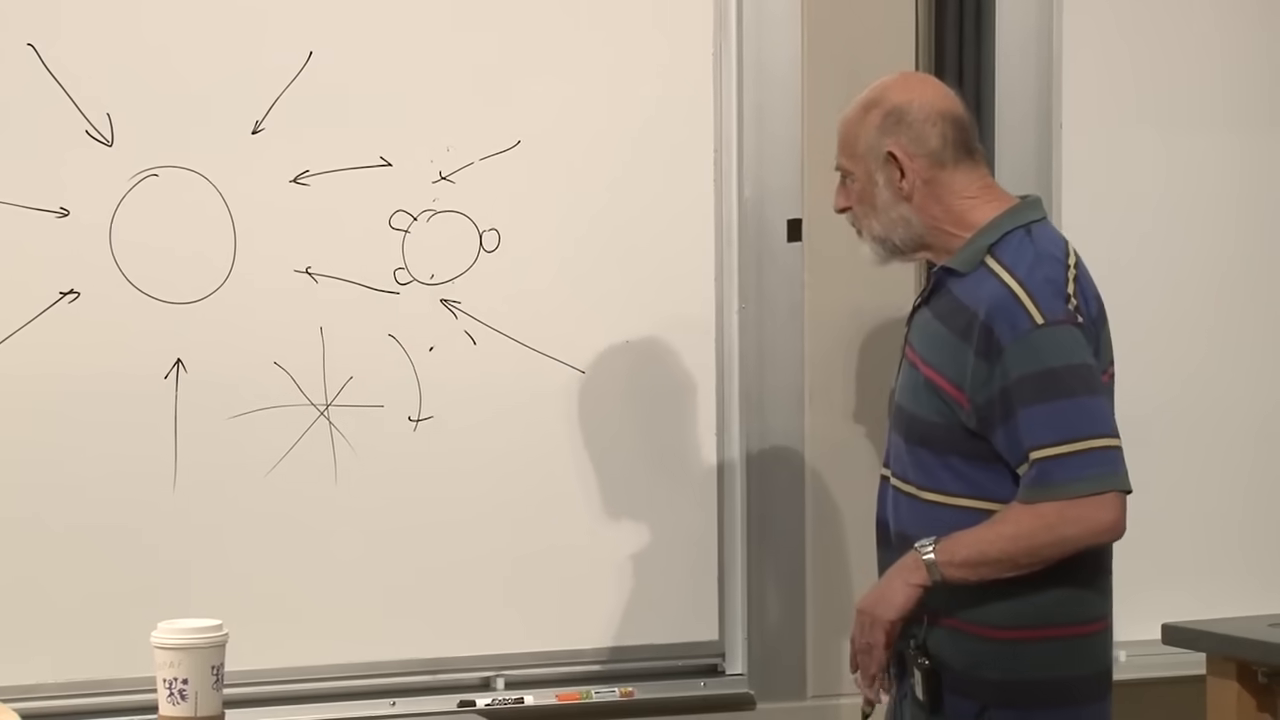
\includegraphics[width=\linewidth]{lecture_01_figure_09.png}
\caption{広がりをもつ自由落下物体について、動径方向の引き伸ばしと横方向の圧縮を同時に示したもの。}
\par\smallskip
\textit{講義フレーム: 00:47:55。}
\end{figure}

\begin{classroomqa}
\audiencequestion{潮汐力は等価原理が破れることを意味するのか。}
\lecturerresponse{それらは、等価原理をどれほど注意深く述べなければならないかを決める。重力場がその内部で無視できるほどしか変化しないほど十分小さな系では、重力は自由落下系によって関連する精度まで取り除くことができる。より大きな系にわたる残りの変化が潮汐場である。\lecturetimestamp{00:48:08}}
\end{classroomqa}

\section{ミンコフスキー幾何から局所計量へ}

ここでいったん重力から離れる。ミンコフスキーはすでに、時空が不変な局所幾何をもつことを教えていた。一次元の空間では、\(c=1\)として、
\begin{equation}
 d\tau^2=dt^2-dx^2.
\label{eq:minkowski-proper-time}
\end{equation}
代わりに\(ds^2=dx^2-dt^2=-d\tau^2\)を定義してもよい。その違いは符号規約の違いであり、物理の違いではない。

\begin{classroomqa}
\audiencequestion{光速を1に設定しない場合、光速はどこに属するのか。}
\lecturerresponse{\(t\)が時間の単位で測られ、\(x\)が長さの単位で測られるなら、一つの便利な形は
\(d\tau^2=dt^2-dx^2/c^2\)である。同値なことに、\(c^2\)を掛けて
\(c^2d\tau^2=c^2dt^2-dx^2\)を用いてもよい。\(ct\)または\(x/c\)を座標として選ぶことは、換算係数を吸収する。\lecturetimestamp{00:51:02}}
\end{classroomqa}

\begin{figure}[H]
\centering
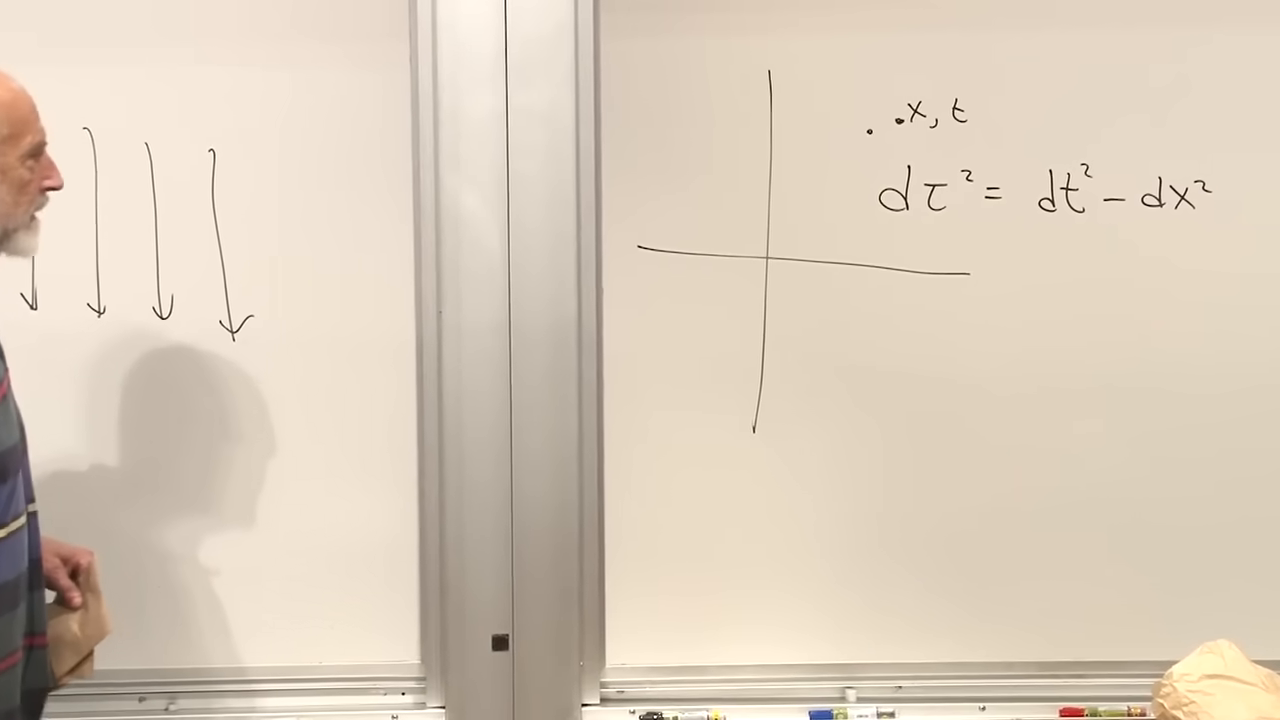
\includegraphics[width=\linewidth]{lecture_01_figure_10.png}
\caption{特殊相対性理論から一般相対性理論への幾何学的な橋を提供する固有時間間隔。}
\par\smallskip
\textit{講義フレーム: 00:51:10。}
\end{figure}

アインシュタインは、重力場が取り除けるかどうかを決める問題が、ガウスが曲面について、リーマンが任意次元で研究した問題に似ていることを認識した。すなわち、局所的な距離の法則が与えられたとき、その幾何が真に曲がっているかどうかをどのように決められるか、という問題である。

ユークリッドのデカルト座標では、ピタゴラスにより
\begin{equation}
 ds^2=(dx^1)^2+(dx^2)^2+\cdots
     =\delta_{mn}\,dx^m dx^n.
\label{eq:euclidean-line-element}
\end{equation}
添字の範囲は空間の次元である。座標が二つ、三つ、二十六個のいずれであっても、記法の中身は変わらない。

\begin{figure}[H]
\centering
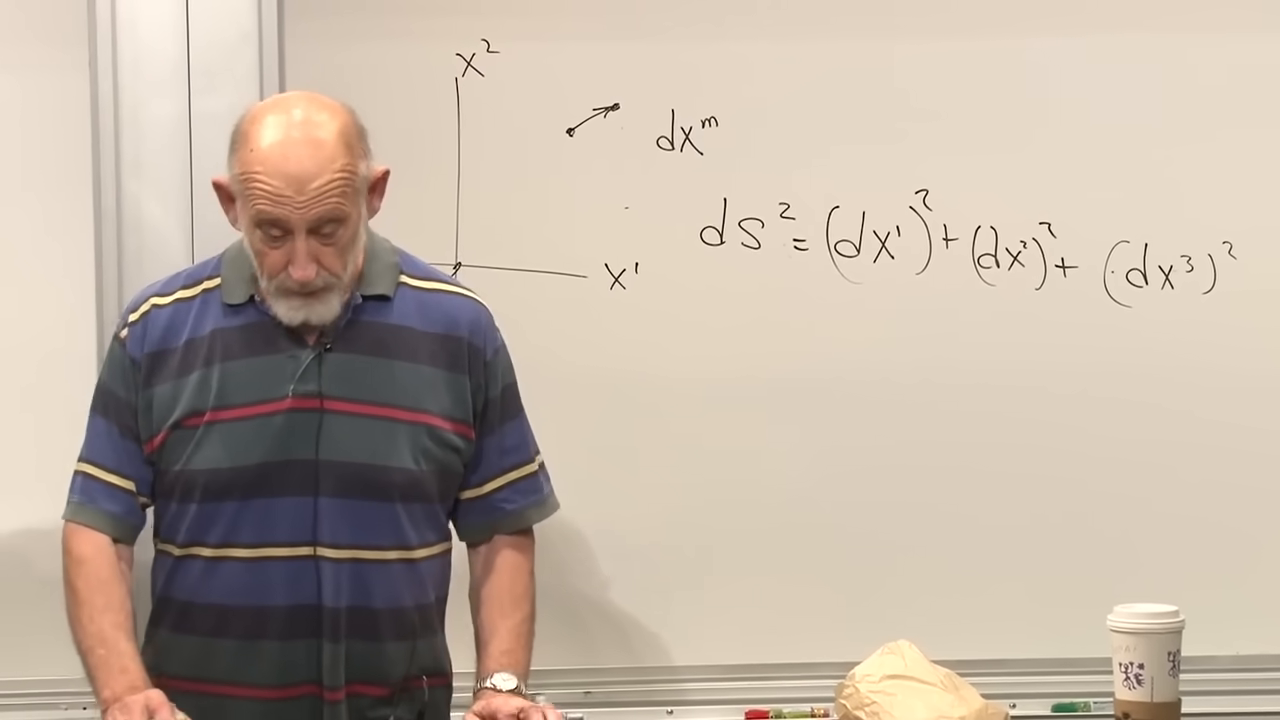
\includegraphics[width=\linewidth]{lecture_01_figure_11.png}
\caption{座標増分の二乗の和としてのユークリッド線素。}
\par\smallskip
\textit{講義フレーム: 00:55:00。}
\end{figure}

任意の曲面に任意の座標\(x^m\)を置く。隣接する点の間の距離は二次形式
\begin{equation}
 ds^2=g_{mn}(x)\,dx^m dx^n.
\label{eq:general-line-element}
\end{equation}
である。関数\(g_{mn}(x)\)は計量テンソルの成分である。同じ式は、曲線座標で記述された平坦な曲面にも当てはまる。計量成分が定数でないこと自体は、内在的曲率を証明しない。

\begin{figure}[H]
\centering
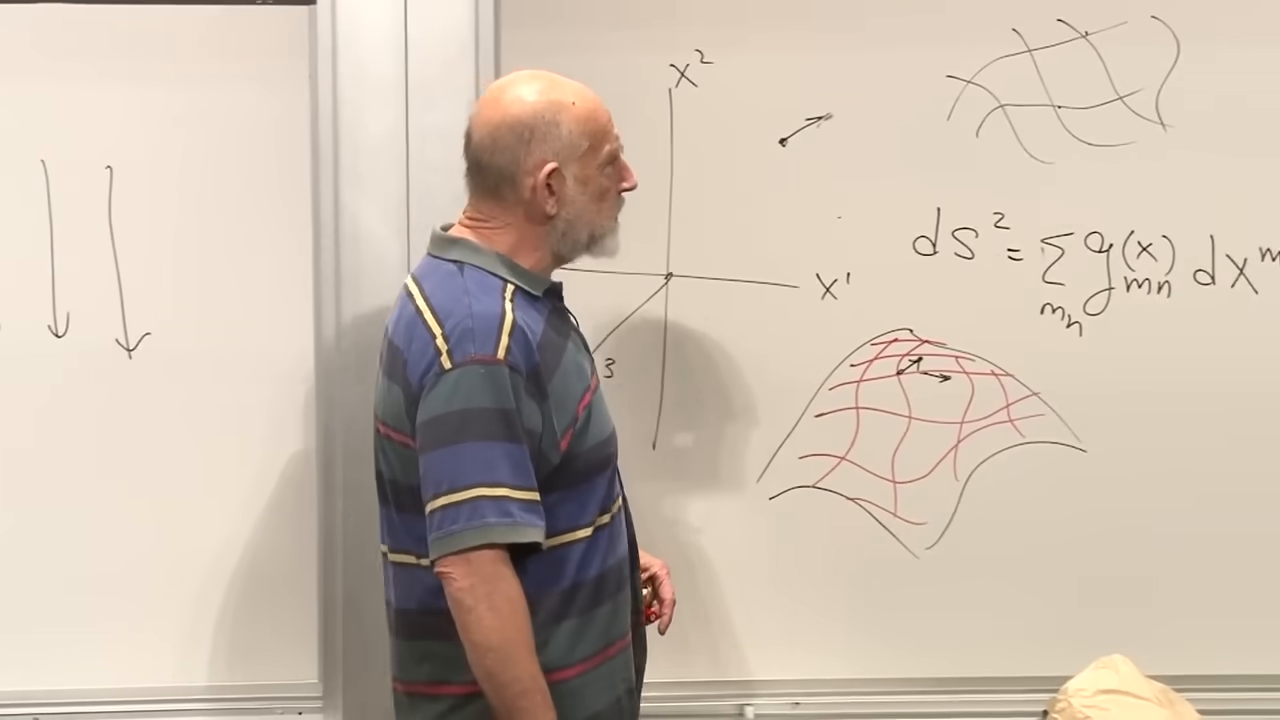
\includegraphics[width=\linewidth]{lecture_01_figure_12.png}
\caption{曲がった座標網の隣に置かれた一般的な計量二次形式。}
\par\smallskip
\textit{講義フレーム: 00:58:20。}
\end{figure}

半径\(R\)の球について、\(\theta\)を極から測ると、
\begin{equation}
 ds^2=R^2\left(d\theta^2+\sin^2\theta\,d\phi^2\right).
\label{eq:sphere-polar}
\end{equation}
同じ経度の増分は、赤道付近では大きな距離を覆い、極付近では小さな距離を覆う。その位置依存性こそが、係数が記録しているものである。

\begin{classroomqa}
\audiencequestion{通常の緯度は赤道から測られるので、係数は正弦ではなく余弦であるべきではないか。}
\lecturerresponse{そのとおりである。\(\lambda\)が赤道から測った緯度を表すならば、
\(ds^2=R^2(d\lambda^2+\cos^2\lambda\,d\phi^2)\)となる。
式\eqref{eq:sphere-polar}では、北極から測った極角
\(\theta=\pi/2-\lambda\)を用いている。
\lecturetimestamp{01:01:03}}
\end{classroomqa}

\begin{figure}[H]
\centering
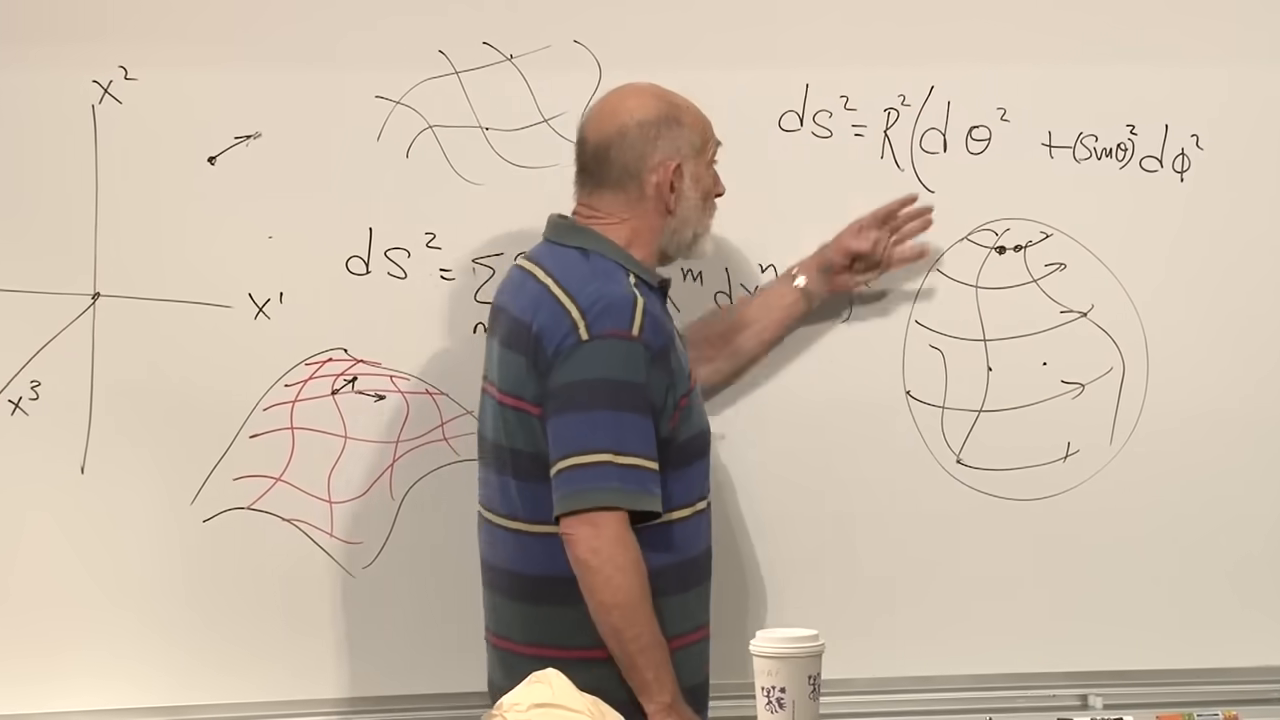
\includegraphics[width=\linewidth]{lecture_01_figure_13.png}
\caption{球面計量と、その位置依存の係数を定める緯度--経度の幾何である。}
\par\smallskip
\textit{講義フレーム：01:00:30。}
\end{figure}

より一般の座標では\(d\theta\,d\phi\)の交差項が現れうるが、局所的な距離は依然として微分の二次式である。三次項や一次項はリーマン線素に属さない。

\section{局所距離と内在的曲率}

\begin{classroomqa}
\audiencequestion{計量の公式は、大きく離れた二点間の距離も与えるのか。}
\lecturerresponse{直接代入によってではない。それは隣接する点の間の距離を与える。巨視的な距離には経路と\(ds\)の積分が必要であり、距離が最短経路を意味するならば、その経路自体を幾何から見出さなければならない。同じ端点を結ぶ局所的最短経路が複数存在することさえある。\lecturetimestamp{01:02:30}}
\end{classroomqa}

起伏のある面上で、離れた二点に杭を打ち、その間に張った糸を想像せよ。糸は丘の一方の側を回ることも他方の側を回ることもあり、丘を動かせば最短経路も変わる。大域的な距離はその間の幾何に依存する。局所的な距離はより単純である。計量は各点に小さな棒を与え、幾何はそれらの無限小の棒から組み立てられる。

\begin{figure}[H]
\centering
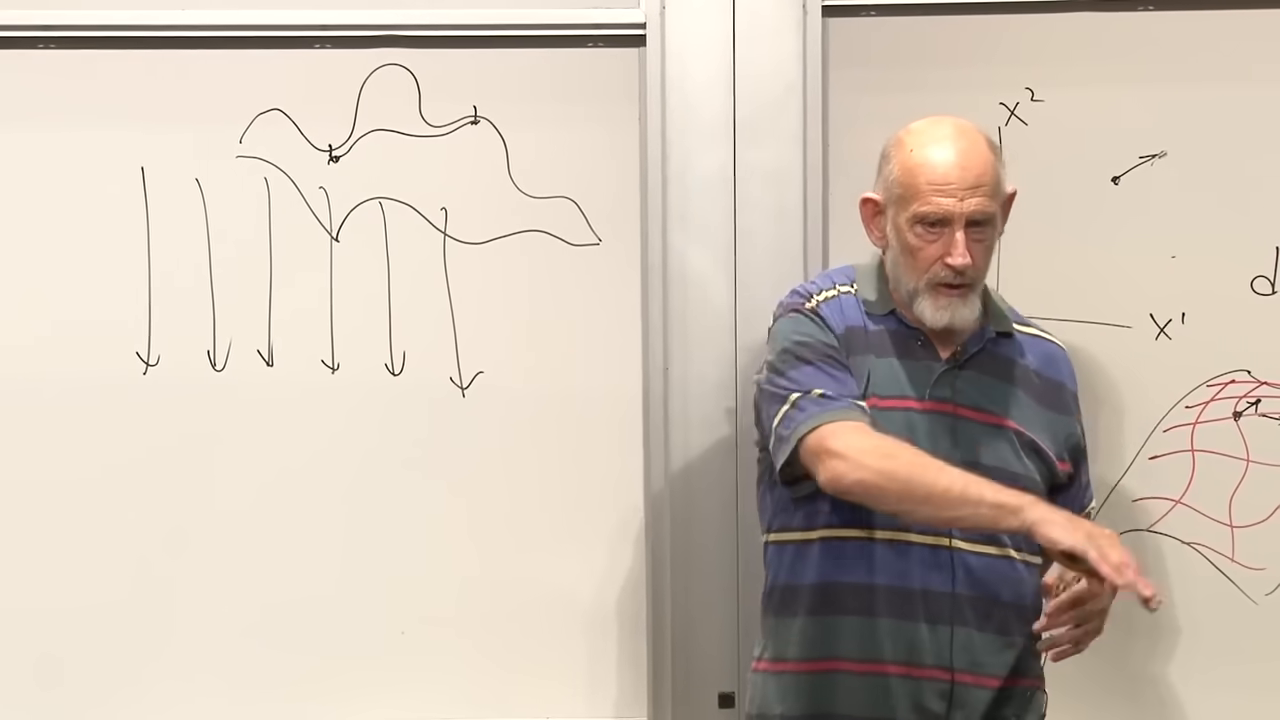
\includegraphics[width=\linewidth]{lecture_01_figure_14.png}
\caption{大域距離の問題：張られた経路は端点の間の面を縫って進まなければならない。}
\par\smallskip
\textit{講義フレーム：01:04:00。}
\end{figure}

局所的な断片を伸縮も破断もなく平面に置くことができるならば、内在的幾何は平坦である。三角分割された球面の長さをもつ断片は、その辺を保ったまますべてを平らに置くことはできない。したがって計量は精密な問題を提起する。\(g_{mn}(x)\)が与えられたとき、その無限小の断片が平坦空間として整合するかどうかを判定できるか。

\begin{figure}[H]
\centering
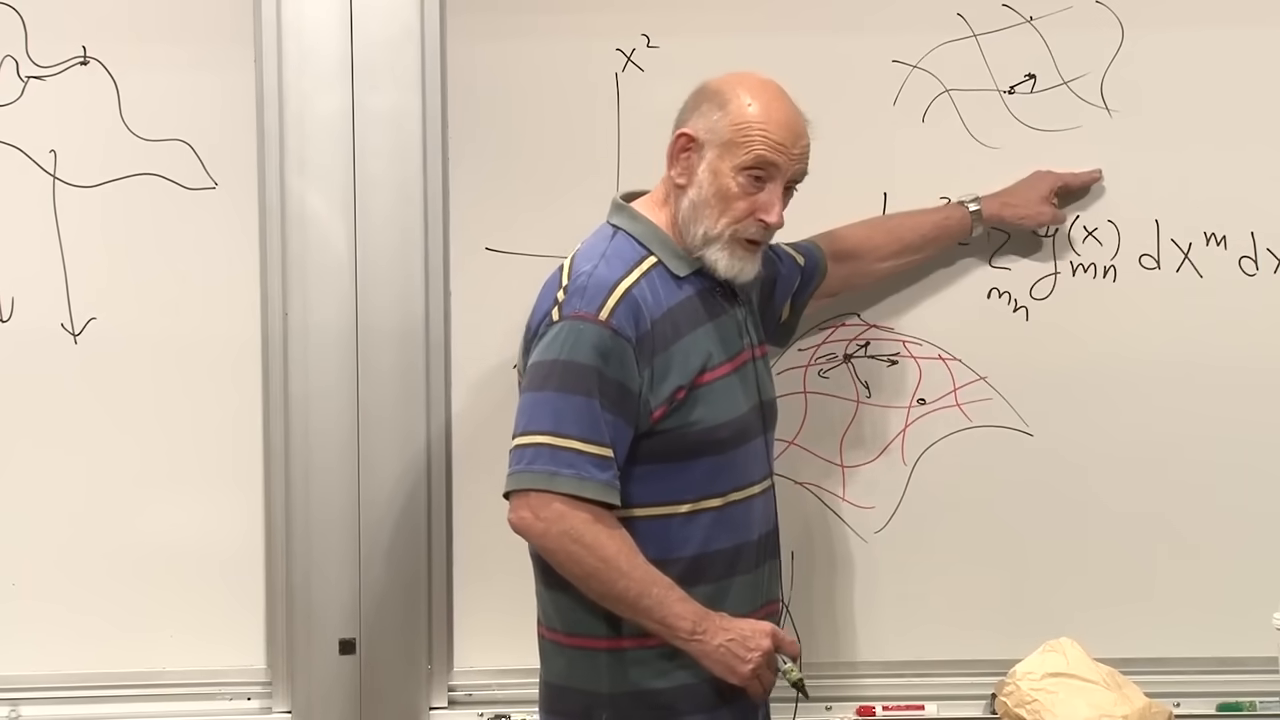
\includegraphics[width=\linewidth]{lecture_01_figure_15.png}
\caption{計量と局所座標パッチを、幾何が組み立てられる無限小の断片として解釈したもの。}
\par\smallskip
\textit{講義フレーム：01:05:20。}
\end{figure}

\begin{classroomqa}
\audiencequestion{円周と直径の比を測ることで曲率を診断できるか。}
\lecturerresponse{できる。それは有用な二次元の判定法である。曲面上ではその比は\(\pi\)と異なりうる。しかし無限小の円では偏差は高次に現れ、この方法は曲率テンソルほどきれいには一般化されない。
\lecturetimestamp{01:07:26}}
\end{classroomqa}

ある領域が平坦であるとは、その領域全体で
\begin{equation}
 g_{mn}=\delta_{mn},
\qquad
 ds^2=\delta_{mn}\,dx^m dx^n
\label{eq:flat-metric}
\end{equation}
となる座標系が存在する場合である。したがって複雑な\(g_{mn}(x)\)は、曲がった空間を記述する場合もあれば、平坦空間上の単に曲がった座標を記述する場合もある。問題は、座標変換によって複雑さをすべて取り除けるかどうかである。

\begin{figure}[H]
\centering
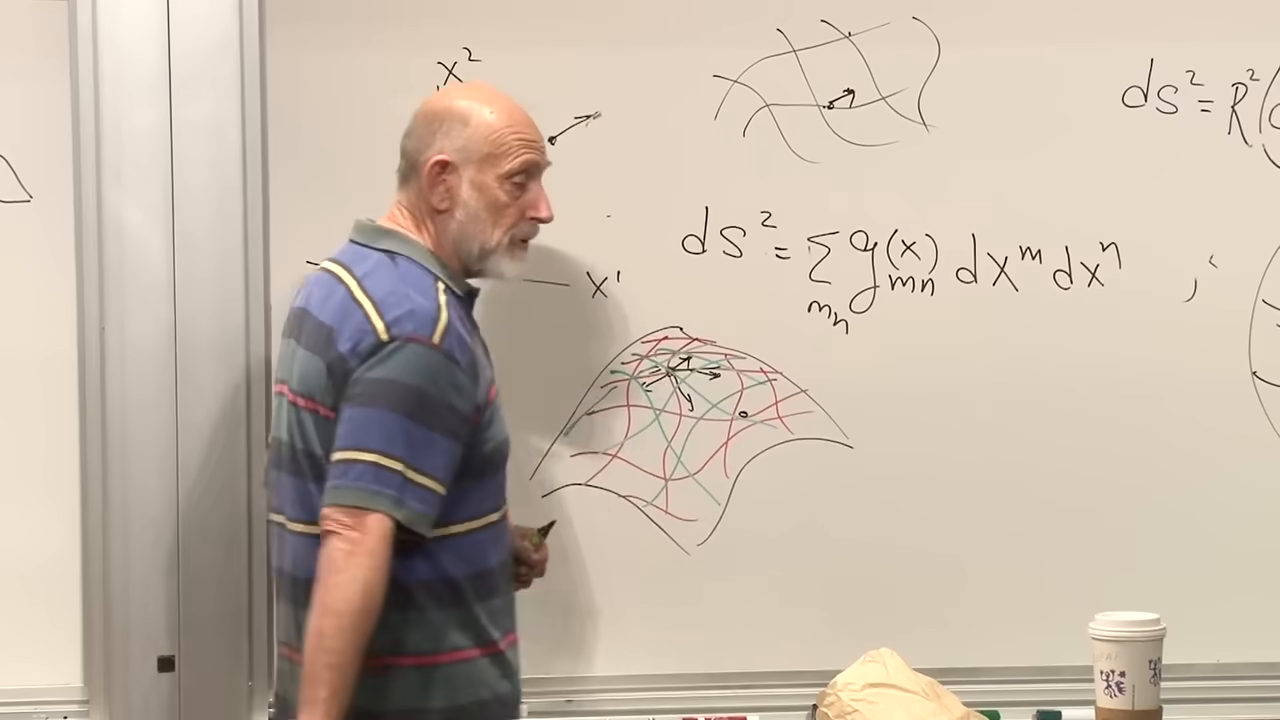
\includegraphics[width=\linewidth]{lecture_01_figure_16.png}
\caption{局所座標パッチ上で述べた計量の問題：その曲線的な形を平坦な形に変換できるか。}
\par\smallskip
\textit{講義フレーム：01:07:15。}
\end{figure}

\begin{classroomqa}
\audiencequestion{球面線素は、球面が平坦でないにもかかわらず、各微小区間が平坦であると仮定しているのか。}
\lecturerresponse{主要次数では、すべての滑らかな曲面は一点においてその接平面で近似される。曲率は、隣接する接平面近似が整合しない仕方に、あるいは有限のパッチにわたる高次の変化に現れる。したがって局所的なユークリッド的振る舞いと大域的な曲率は両立する。\lecturetimestamp{01:10:01}}
\end{classroomqa}

\begin{classroomqa}
\audiencequestion{計量は連続でなければならないのか。折り目や裂け目では何が起こるのか。}
\lecturerresponse{この議論は、必要な導関数に足る滑らかさをもつ座標写像と計量を仮定している。伸縮なしに折られた紙は、折り目の両側で同じ内在的距離をもつ。その劇的な外観は外在的である。真に特異な、あるいは滑らかでない幾何には別個の注意が必要であり、ここで用いた滑らかな設定の範囲外である。\lecturetimestamp{01:11:25}}
\end{classroomqa}

この区別が内在的幾何である。三次元空間で紙を曲げるとその埋め込みは変わるが、紙の内部で測られる距離は変わらない。埋め込み空間を覗くことのできない、紙に閉じ込められた生き物でも、その内在的幾何を測ることはできる。

\begin{figure}[H]
\centering
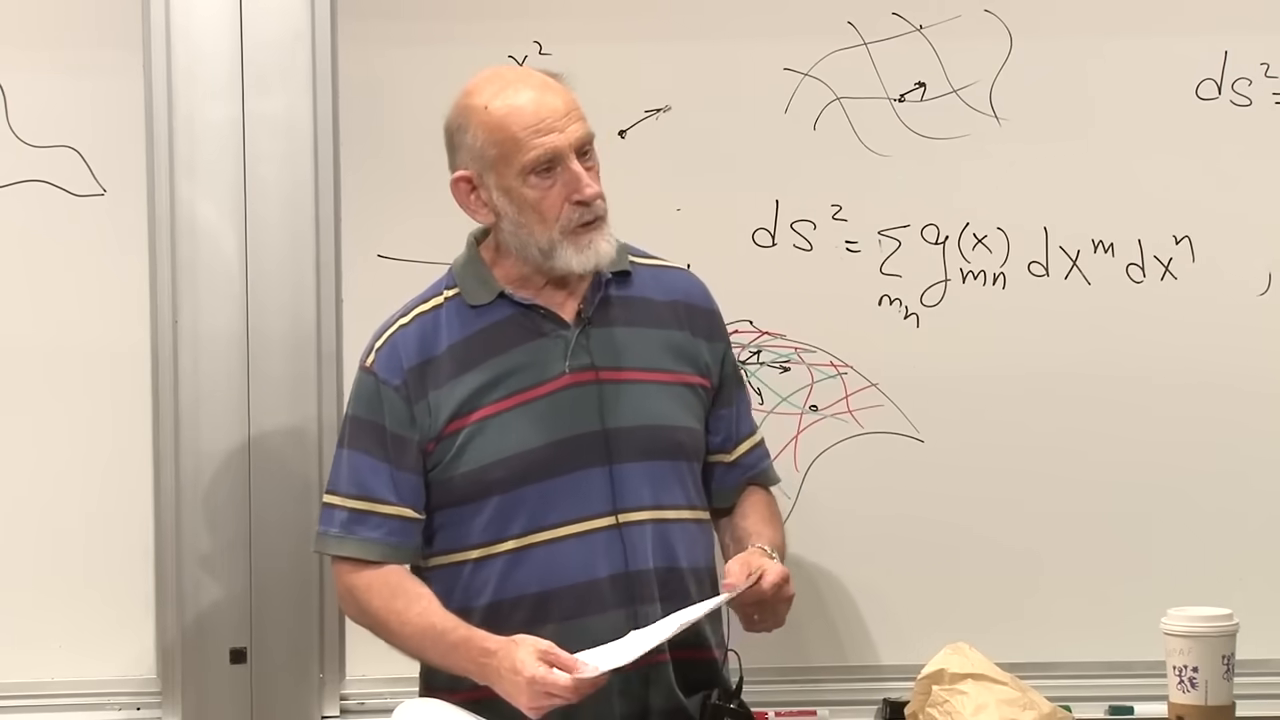
\includegraphics[width=\linewidth]{lecture_01_figure_17.png}
\caption{内在的な距離を外見的な見え方から分離するために用いられる折り畳まれた紙。}
\par\smallskip
\textit{講義フレーム：01:13:00。}
\end{figure}

\begin{classroomqa}
\audiencequestion{なぜ単に計量を対角化しないのか。}
\lecturerresponse{任意の一点では、適切な座標の選び方によって計量を対角化し、局所的な平坦な形に規格化することができる。障害となるのは、一つの座標系で領域全体にわたってそうすることである。曲率は一点だけを調べても検出できない。
\lecturetimestamp{01:13:48}}
\end{classroomqa}

\begin{figure}[H]
\centering
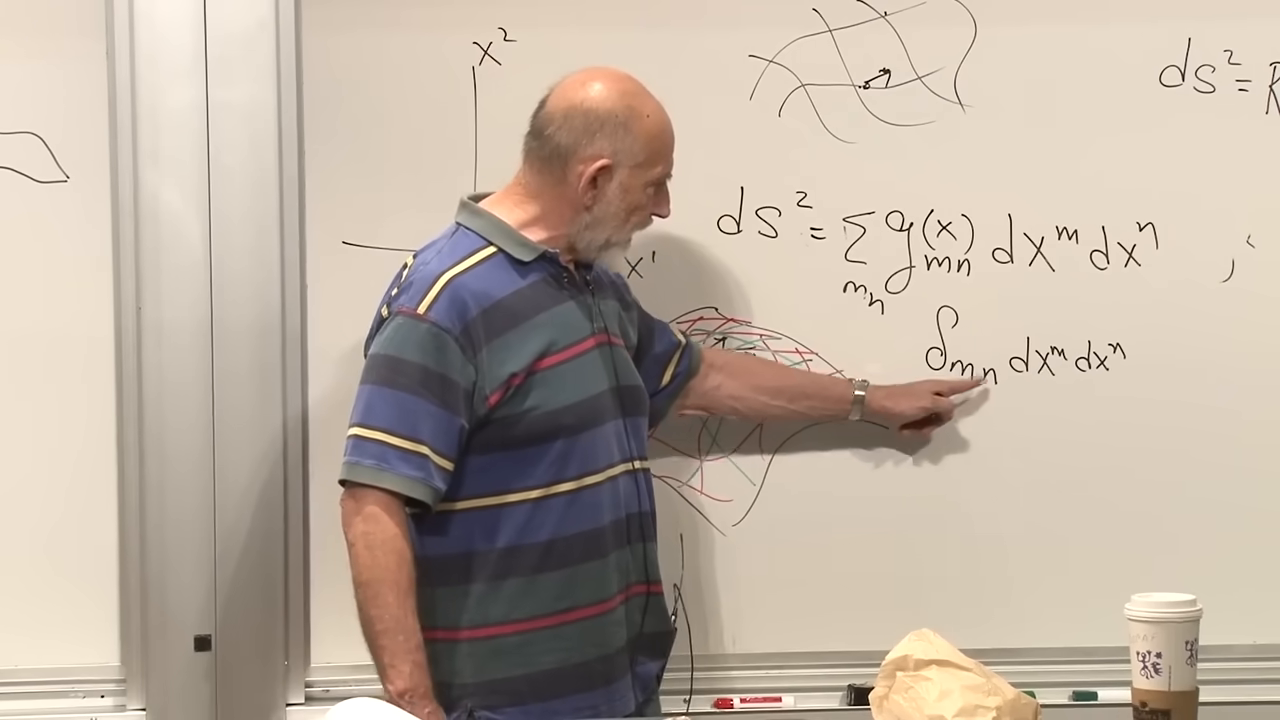
\includegraphics[width=\linewidth]{lecture_01_figure_18.png}
\caption{一般的な局所二次形式の下に書かれた平坦なデカルト計量\(\delta_{mn}\)。}
\par\smallskip
\textit{講義フレーム：01:16:00。}
\end{figure}

重力との類似は今や示唆的ではなく正確である。座標力が除去可能であるのとちょうど同じように、平坦空間の曲線的な記述も除去可能である。潮汐加速度は一般相対性理論では曲率によって測定される。後の記法では、隣接する自由落下世界線は測地線偏差方程式を満たす
\begin{equation}
 \frac{D^2\xi^\mu}{D\tau^2}
 =-R^\mu{}_{\nu\rho\sigma}
   u^\nu\xi^\rho u^\sigma.
\label{eq:geodesic-deviation-preview}
\end{equation}
曲率が消えることは不変な潮汐場がないことを意味し、曲率が非零であることは、その領域全体にわたって重力を除去できる座標の選び方が存在しないことを意味する。

\section{二つの座標系と一つのベクトル}

計量を\(\delta_{mn}\)に変換できるかどうかを決めるには、まず幾何学的対象がどのように変換するかを知らなければならない。\(x^m\)と\(y^m\)を同じ領域上の二つの滑らかな座標系とする：
\begin{equation}
 x^m=x^m(y),\qquad y^m=y^m(x).
\label{eq:mutual-coordinate-maps}
\end{equation}
記号\(x\)と\(y\)は完全な座標系を表し、二つの特定の空間方向を表すのではない。

\begin{figure}[H]
\centering
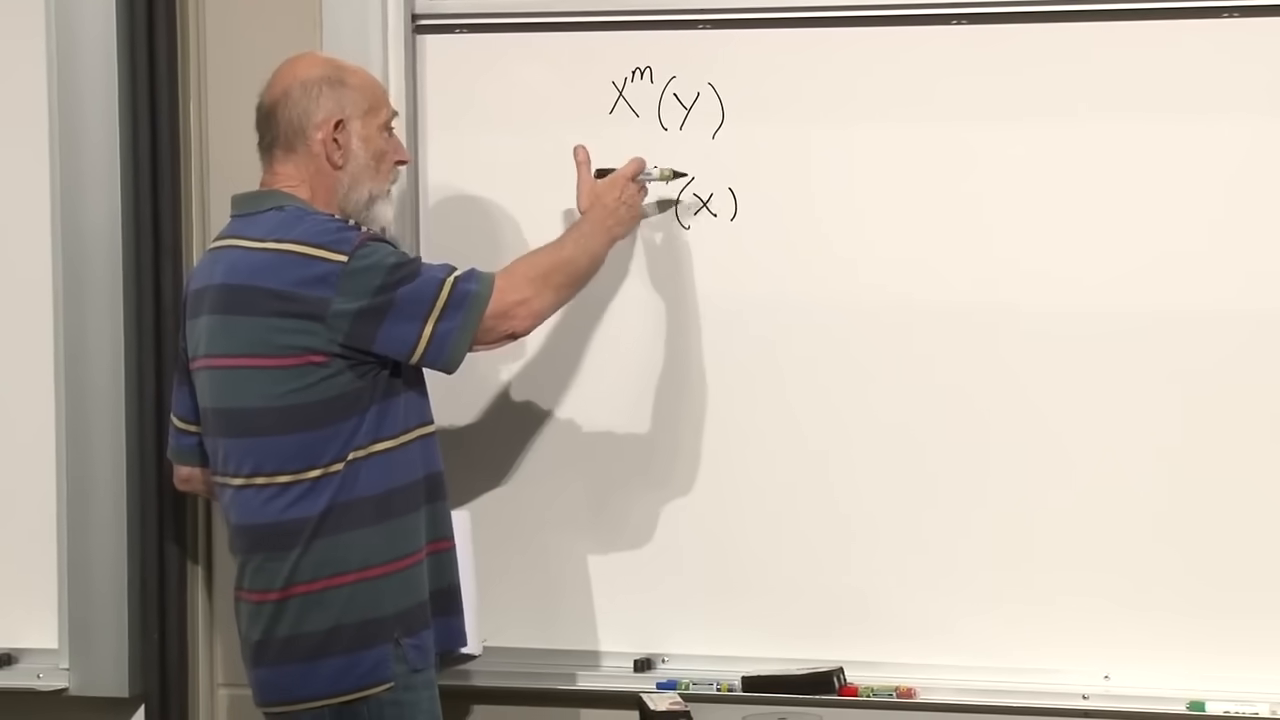
\includegraphics[width=\linewidth]{lecture_01_figure_19.png}
\caption{互いに関連する座標写像\(x^m(y)\)と\(y^m(x)\)。}
\par\smallskip
\textit{講義フレーム：01:20:35。}
\end{figure}

隣接する点に対して、連鎖律は次を与える
\begin{equation}
 dy^m=\frac{\partial y^m}{\partial x^p}\,dx^p.
\label{eq:differential-transform}
\end{equation}
繰り返された添字\(p\)は和をとる。変位それ自体は一つの幾何学的ベクトルであり、\(dx^p\)と\(dy^m\)は二つの座標系におけるその成分である。

\begin{figure}[H]
\centering
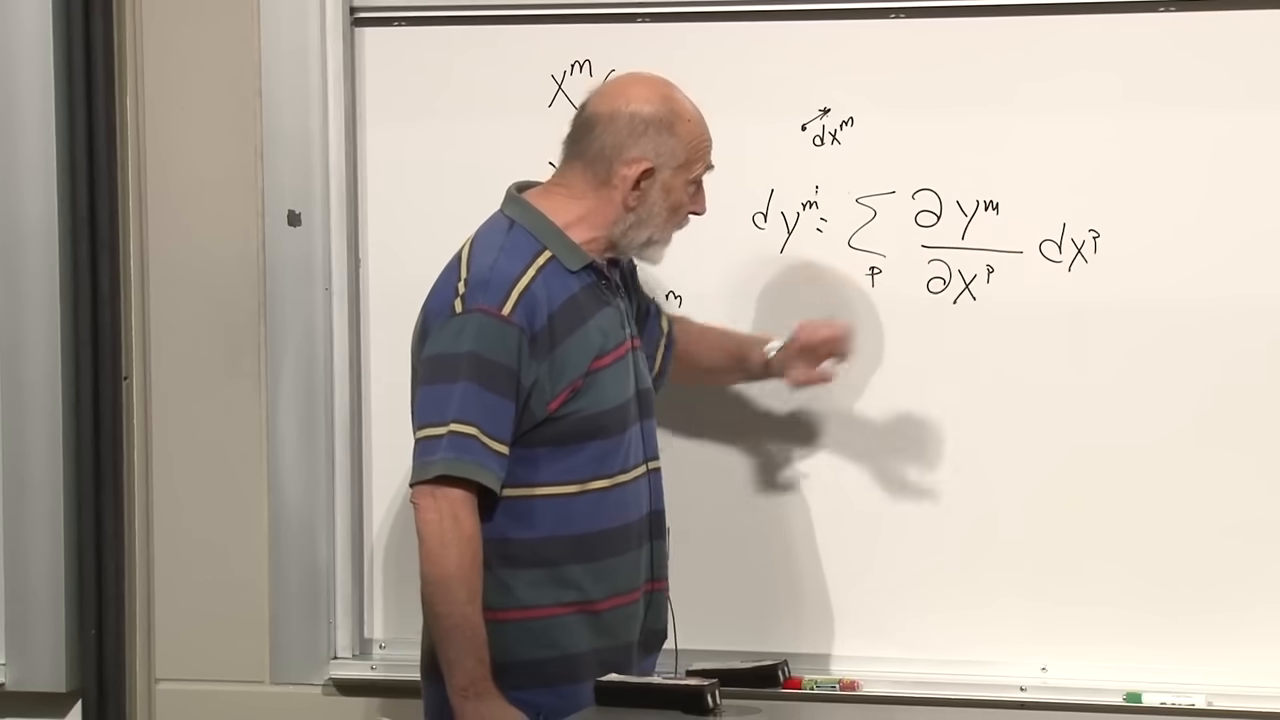
\includegraphics[width=\linewidth]{lecture_01_figure_20.png}
\caption{連鎖律から得られる微分座標変換。}
\par\smallskip
\textit{講義フレーム：01:22:30。}
\end{figure}

\begin{classroomqa}
\audiencequestion{曲線的な格子では、座標線は何を表すのか。}
\lecturerresponse{二次元では、一方の座標を固定して他方を変化させることによって線が得られる。より高次元では、対応する定座標集合は超曲面である。それらの局所的な交わりが、ベクトル成分を分解するために用いられる座標方向を定義する。\lecturetimestamp{01:25:20}}
\end{classroomqa}

反変ベクトルは座標変位と同じ変換則によって定義される：
\begin{equation}
 (V')^m(y)
 =\frac{\partial y^m}{\partial x^p}\,V^p(x).
\label{eq:contravariant-vector}
\end{equation}
表面上の速度が一例である。座標が変わってもベクトルは変化しない。変化するのはその成分である。

\begin{figure}[H]
\centering
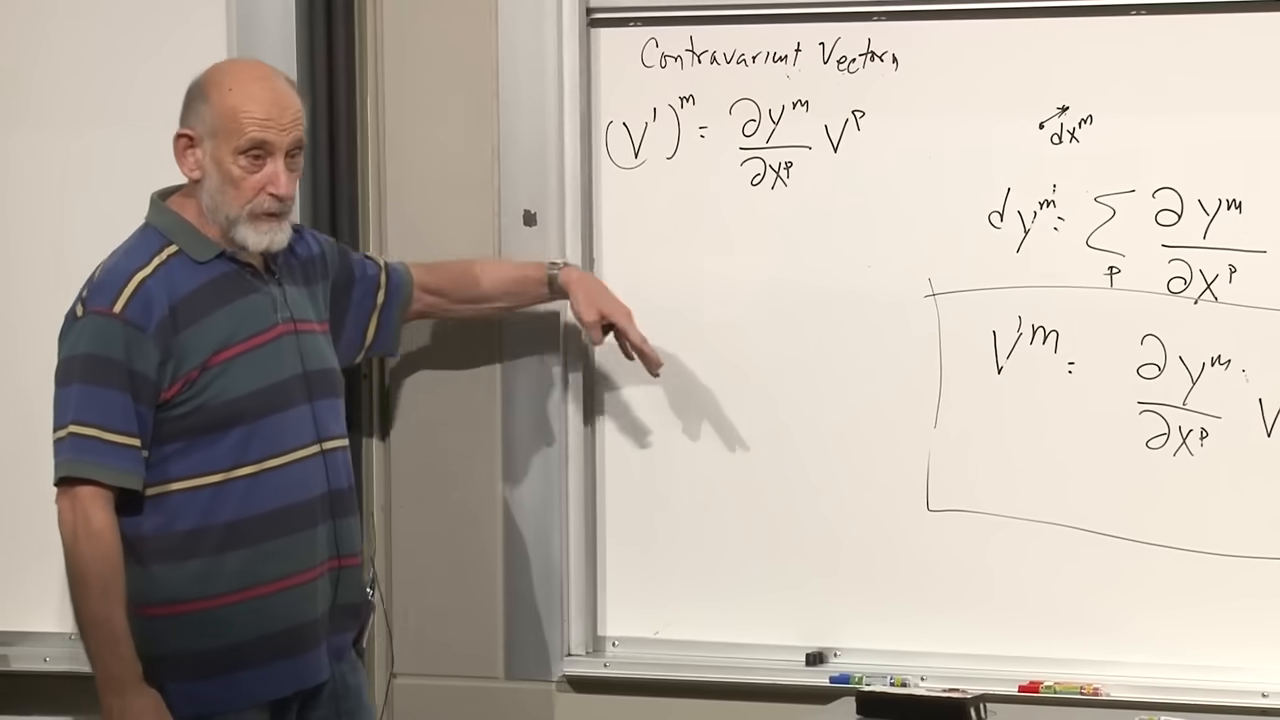
\includegraphics[width=\linewidth]{lecture_01_figure_21.png}
\caption{反変ベクトルの変換則を枠で囲んだもの。}
\par\smallskip
\textit{講義フレーム：01:29:30。}
\end{figure}

アインシュタインの総和規約は、添字が上に一度、下に一度現れるたびに総和記号を省略する。この規約は数式を印刷しやすくしたが、より重要なのは収縮のパターンを可視化することである。

\begin{classroomqa}
\audiencequestion{どの座標系が許されるかについて特別な仮定が置かれているのか。}
\lecturerresponse{二つの系が関数的に関連しており、議論中の領域で表示された導関数と逆写像が存在するのに十分滑らかであるということだけである。線形性も直交性も仮定されていない。\lecturetimestamp{01:28:12}}
\end{classroomqa}

\section{余ベクトルと連鎖律}

\(S(x)\)をスカラーとする：それは各点で一つのよく定義された値をもち、座標ラベルに依存しない。温度やスカラー場が例である。その勾配は成分
\begin{equation}
 W_p=\frac{\partial S}{\partial x^p}.
\label{eq:gradient-covector}
\end{equation}
をもつ。

\begin{figure}[H]
\centering
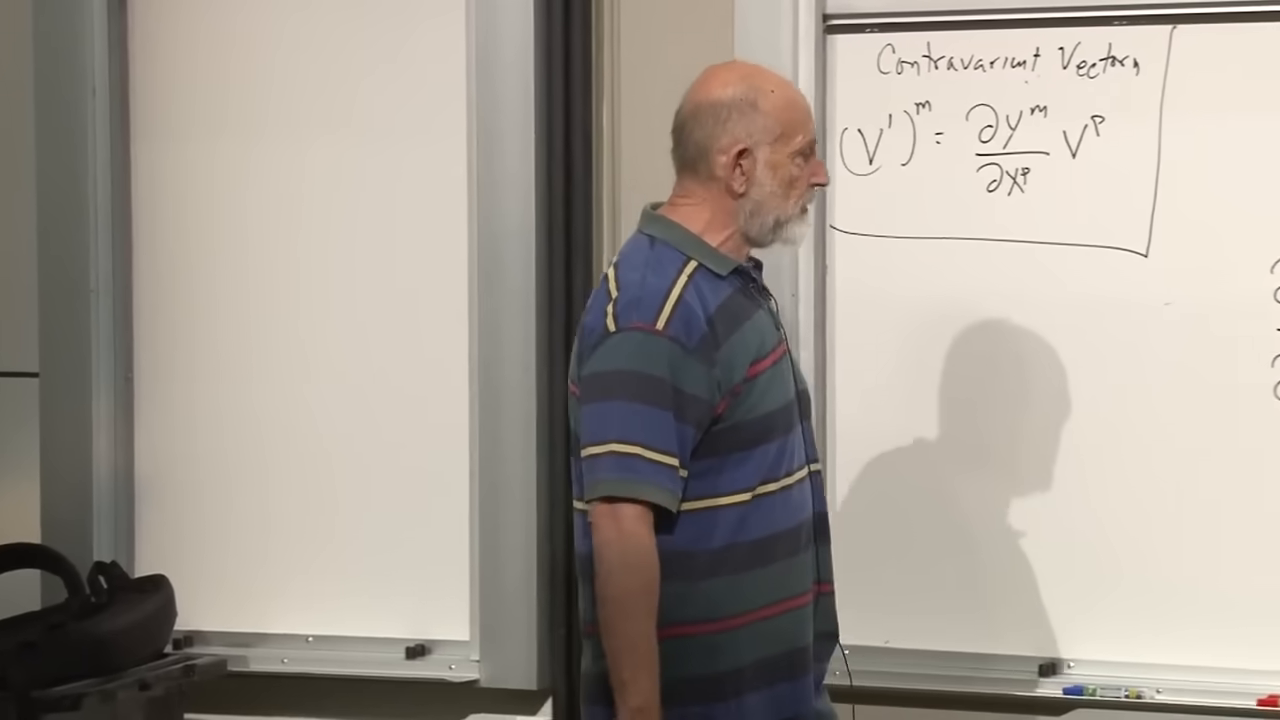
\includegraphics[width=\linewidth]{lecture_01_figure_22.png}
\caption{反変変換則の隣に導入されたスカラー勾配。}
\par\smallskip
\textit{講義フレーム：01:31:40。}
\end{figure}

\(y\)座標で連鎖律を適用すると、
\begin{equation}
 W'_m
 =\frac{\partial S}{\partial y^m}
 =\frac{\partial x^p}{\partial y^m}
  \frac{\partial S}{\partial x^p}
 =\frac{\partial x^p}{\partial y^m}\,W_p.
\label{eq:covariant-vector}
\end{equation}
これが共変ベクトル、すなわち余ベクトルの変換則である。ヤコビアンは\eqref{eq:contravariant-vector}のものの逆であり、したがって下付き添字と上付き添字は異なる変換挙動を表す。

\begin{figure}[H]
\centering
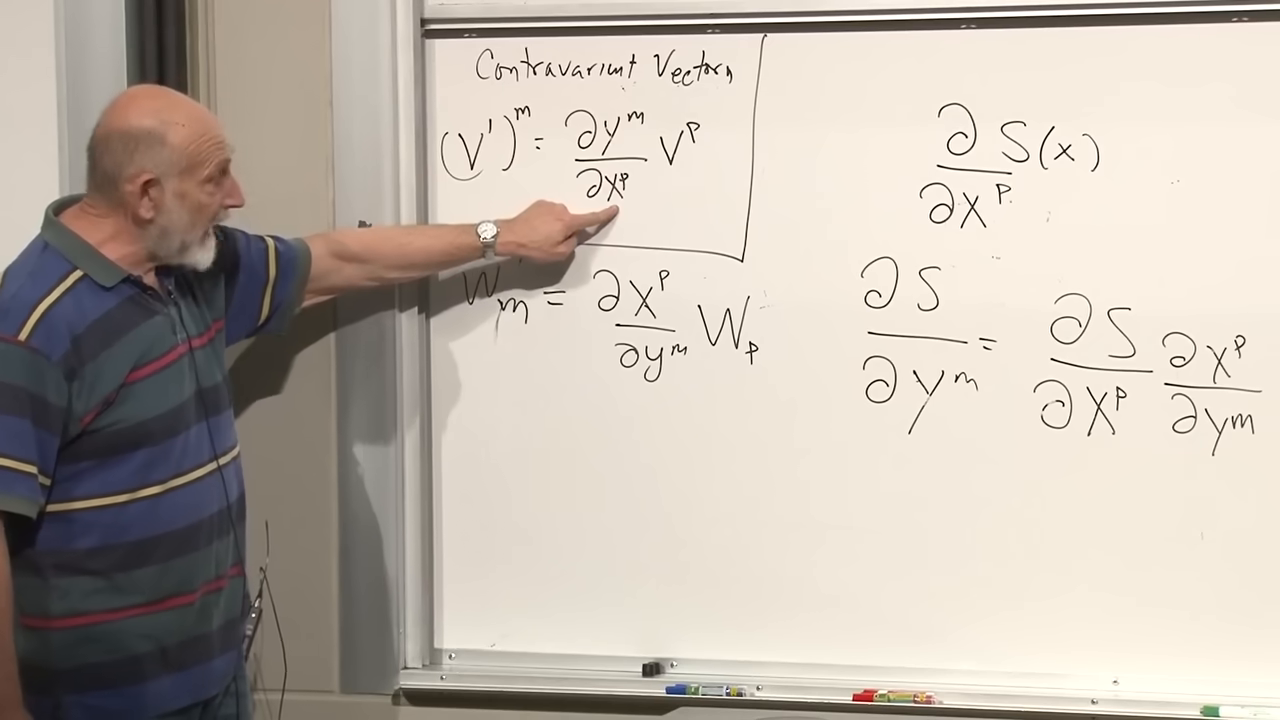
\includegraphics[width=\linewidth]{lecture_01_figure_23.png}
\caption{反変変換則と共変変換則を並べて表示したもの。}
\par\smallskip
\textit{講義フレーム：01:34:40。}
\end{figure}

\begin{classroomqa}
\audiencequestion{共変ベクトルと反変ベクトルの間の関係は何か。}
\lecturerresponse{現段階では、それらは異なる種類の対象として定義されている。すなわち、変位と速度は一方の仕方で変換し、勾配は逆の仕方で変換する。計量は後に、添字を下げたり上げたりする一対一の写像を与えるであろう。その関係は、計量が導入される前に仮定されるべきではない。\lecturetimestamp{01:37:43}}
\end{classroomqa}

\begin{classroomqa}
\audiencequestion{以前に添字を下げると時間成分の符号が変わったのではないか。}
\lecturerresponse{その符号はローレンツ計量から来たものである。現在の導出はまず通常のユークリッド幾何学で行われている。添字の上げ下げは常に該当する計量を用いる。時間成分の符号は、その計量がローレンツ的符号数を持つ場合にのみ現れる。
\lecturetimestamp{01:38:29}}
\end{classroomqa}

\begin{classroomqa}
\audiencequestion{二つの変換則は、すでに同じベクトルの二つの成分記述と見なされるべきか。}
\lecturerresponse{まだそうではない。計量が利用可能になれば、反変ベクトル\(V^m\)を共ベクトル\(V_m=g_{mn}V^n\)に変換できる。その写像が確立されるまでは、上付き添字と下付き添字の対象は論理的に別個のものである。\lecturetimestamp{01:39:00}}
\end{classroomqa}

これらの式は次元に依存しない。添字の範囲は変わるが、変換則は変わらない。

\section{複数の添字を持つテンソル}

二つの反変ベクトル\(V^m\)と\(U^n\)を取る。それらの積
\begin{equation}
 T^{mn}=V^mU^n
\label{eq:rank-two-product}
\end{equation}
は二階の反変テンソルである。三次元では九つの成分を持ち、四次元では十六の成分を持つ。別に与えられた対称性がない限り、添字の順序は重要である。\(T^{mn}\)は\(T^{nm}\)に等しい必要はない。

\begin{figure}[H]
\centering
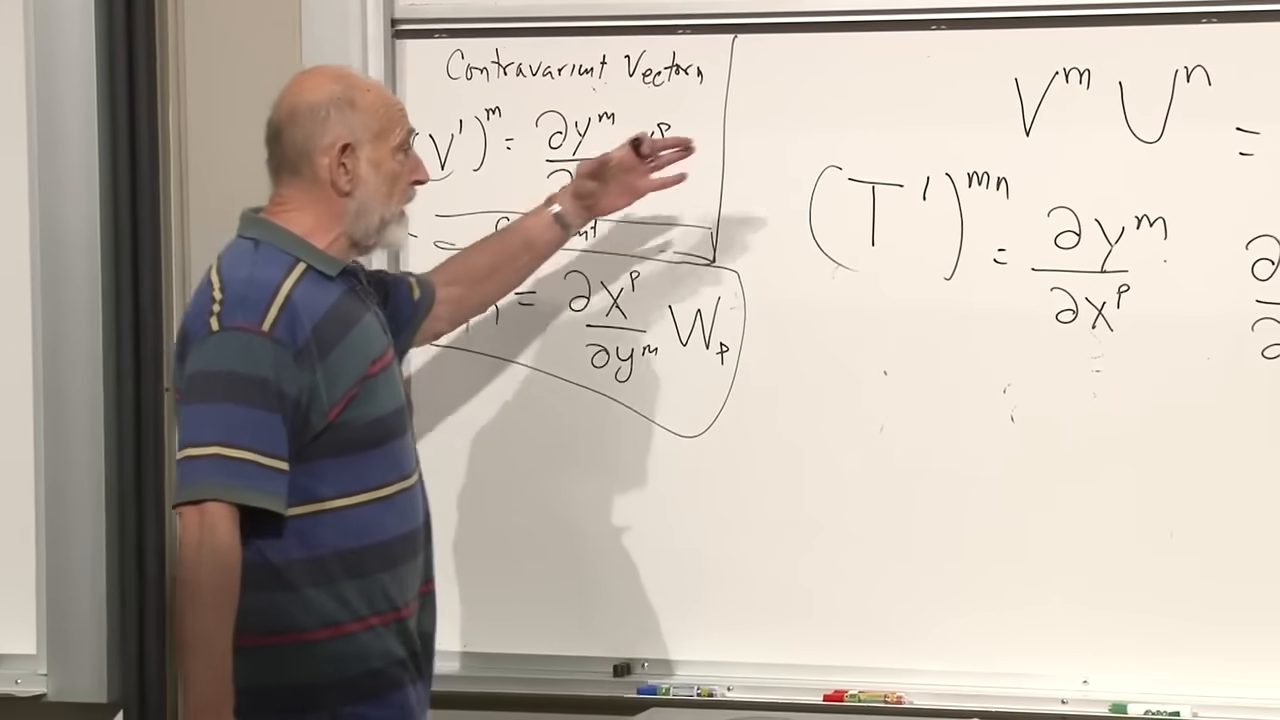
\includegraphics[width=\linewidth]{lecture_01_figure_24.png}
\caption{二つの反変ベクトルの積として構成された二階テンソル。}
\par\smallskip
\textit{講義フレーム：01:43:40。}
\end{figure}

各上付き添字は一つの順ヤコビアンに寄与する：
\begin{equation}
 (T')^{mn}
 =\frac{\partial y^m}{\partial x^p}
  \frac{\partial y^n}{\partial x^q}
  T^{pq}.
\label{eq:rank-two-contravariant}
\end{equation}
積の構成はこの規則を動機づけるが、変換則がテンソルの定義である。三階の反変テンソルはそのようなヤコビアン因子を三つ獲得するであろう。

\begin{figure}[H]
\centering
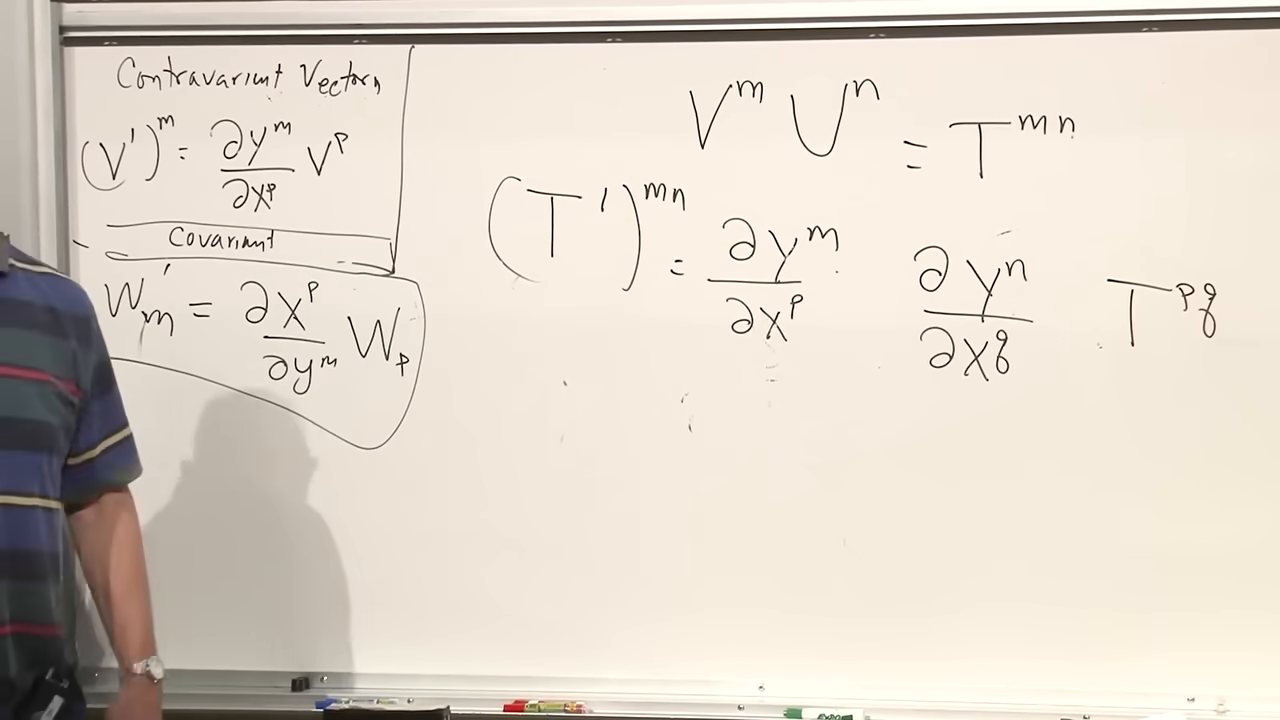
\includegraphics[width=\linewidth]{lecture_01_figure_25.png}
\caption{\(T^{mn}\)の変換における二つのヤコビアン因子。}
\par\smallskip
\textit{講義フレーム：01:44:20。}
\end{figure}

同様に、各下付き添字は一つの逆ヤコビアンに寄与する：
\begin{equation}
 T'_{mn}
 =\frac{\partial x^p}{\partial y^m}
  \frac{\partial x^q}{\partial y^n}
  T_{pq}.
\label{eq:rank-two-covariant}
\end{equation}
混合テンソルは各種類の因子を一つずつ用いる。

\begin{figure}[H]
\centering
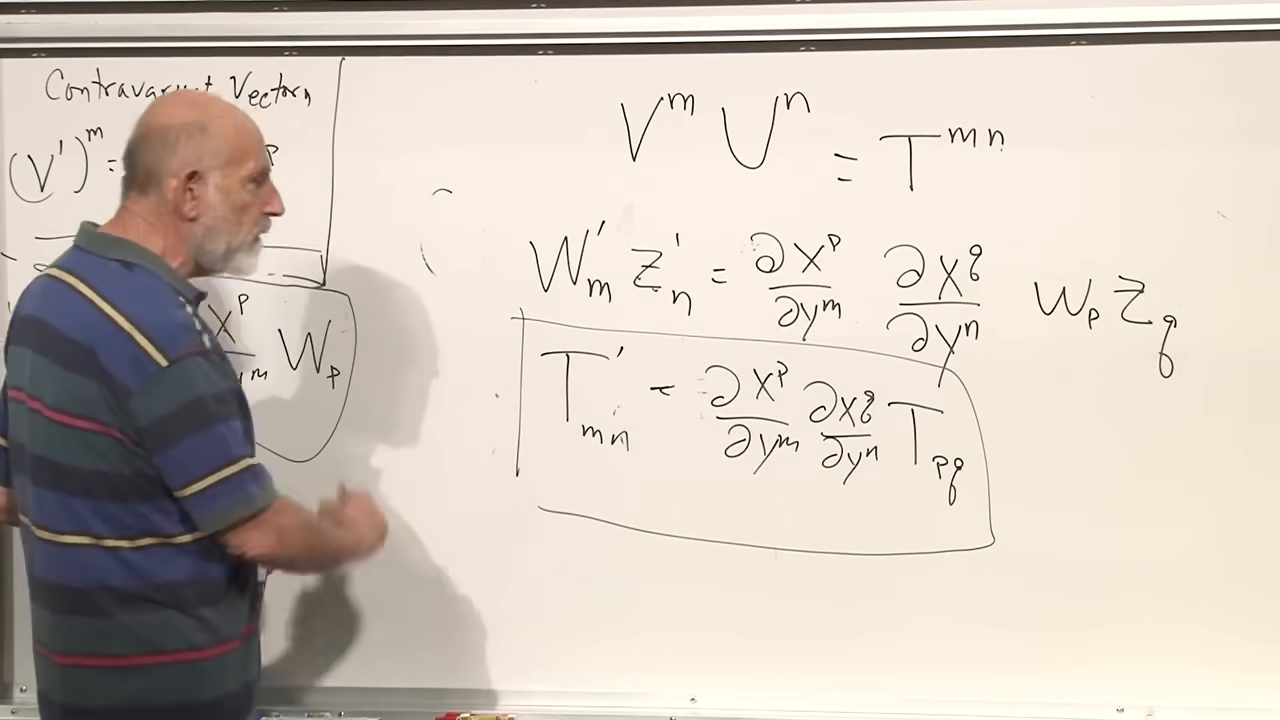
\includegraphics[width=\linewidth]{lecture_01_figure_26.png}
\caption{二つの共変添字を持つテンソルの完成した変換則。}
\par\smallskip
\textit{講義フレーム：01:47:30。}
\end{figure}

同じ変換の仕組みが今や計量に適用される。間隔はスカラーであるから、どちらの座標系でも同じ値を持たなければならない：
\begin{align}
 ds^2
 &=g_{mn}(x)\,dx^m dx^n,\\
 dx^m
 &=\frac{\partial x^m}{\partial y^p}\,dy^p.
\end{align}
代入により、板書が未完成のまま残した行が完成する：
\begin{equation}
 g'_{pq}(y)
 =\frac{\partial x^m}{\partial y^p}
  \frac{\partial x^n}{\partial y^q}
  g_{mn}(x(y)).
\label{eq:l1-metric-transformation}
\end{equation}
したがって\(g_{mn}\)は二階の共変テンソルである。

\begin{figure}[H]
\centering
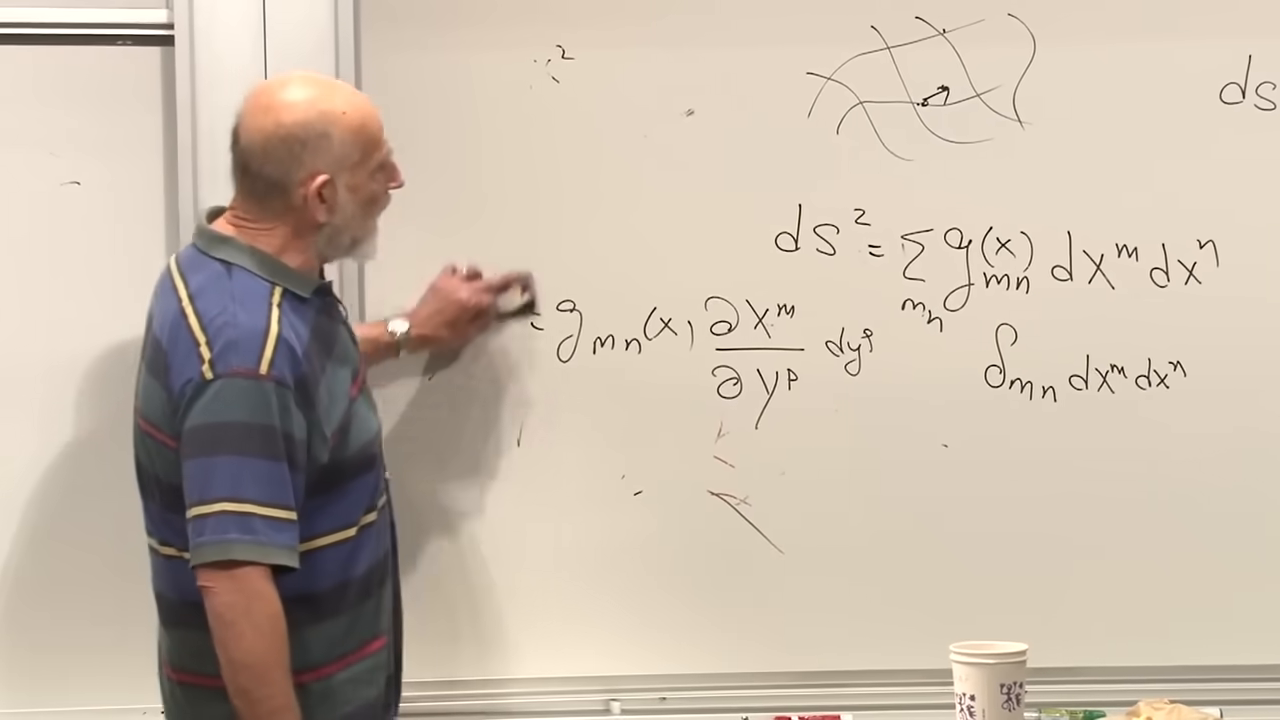
\includegraphics[width=\linewidth]{lecture_01_figure_27.png}
\caption{講義の終わりに線素の不変性から始められた計量の変換。}
\par\smallskip
\textit{講義フレーム：01:48:40。}
\end{figure}

冒頭の物理的な問いは、今や数学的な問いになった。\(g_{mn}(x)\)が与えられたとき、領域全体で\(g'_{mn}=\delta_{mn}\)となるような座標変換は存在するか。もし存在すれば、見かけの複雑さは座標の複雑さにすぎない。もし存在しなければ、その障害は曲率であり、時空においてその障害は重力の不変な内容である。
